%%%%%%%%%%%%%%%%%%%%%%%%%%%%%%%%%%%%%%%%%
% Beamer Presentation
% LaTeX Template
% Version 1.0 (10/11/12)
%
% This template has been downloaded from:
% http://www.LaTeXTemplates.com
%
% License:
% CC BY-NC-SA 3.0 (http://creativecommons.org/licenses/by-nc-sa/3.0/)
%
%%%%%%%%%%%%%%%%%%%%%%%%%%%%%%%%%%%%%%%%%

%----------------------------------------------------------------------------------------
%	PACKAGES AND THEMES
%----------------------------------------------------------------------------------------

\documentclass[xcolor=table]{beamer}

\mode<presentation> {

% The Beamer class comes with a number of default slide themes
% which change the colors and layouts of slides. Below this is a list
% of all the themes, uncomment each in turn to see what they look like.

%\usetheme{default}
%\usetheme{AnnArbor}
%\usetheme{Antibes}
%\usetheme{Bergen}
%\usetheme{Berkeley}
%\usetheme{Berlin}
%\usetheme{Boadilla}
%\usetheme{CambridgeUS}
%\usetheme{Copenhagen}
%\usetheme{Darmstadt}
%\usetheme{Dresden}
%\usetheme{Frankfurt}
%\usetheme{Goettingen}
%\usetheme{Hannover}
%\usetheme{Ilmenau}
%\usetheme{JuanLesPins}
%\usetheme{Luebeck}
\usetheme{Madrid}
%\usetheme{Malmoe}
%\usetheme{Marburg}
%\usetheme{Montpellier}
%\usetheme{PaloAlto}
%\usetheme{Pittsburgh}
%\usetheme{Rochester}
%\usetheme{Singapore}
%\usetheme{Szeged}
%\usetheme{Warsaw}

% As well as themes, the Beamer class has a number of color themes
% for any slide theme. Uncomment each of these in turn to see how it
% changes the colors of your current slide theme.

%\usecolortheme{albatross}
%\usecolortheme{beaver}
%\usecolortheme{beetle}
%\usecolortheme{crane}
%\usecolortheme{dolphin}
%\usecolortheme{dove}
%\usecolortheme{fly}
%\usecolortheme{lily}
%\usecolortheme{orchid}
%\usecolortheme{rose}
%\usecolortheme{seagull}
%\usecolortheme{seahorse}
%\usecolortheme{whale}
%\usecolortheme{wolverine}

%\setbeamertemplate{footline} % To remove the footer line in all slides uncomment this line
%\setbeamertemplate{footline}[page number] % To replace the footer line in all slides with a simple slide count uncomment this line

%\setbeamertemplate{navigation symbols}{} % To remove the navigation symbols from the bottom of all slides uncomment this line
}

\usepackage{graphicx} % Allows including images


%----------------------------------------------------------------------------------------
%	TITLE PAGE
%----------------------------------------------------------------------------------------

\title[Documentation on LOA]{Documentation on Lion Optimization Algorithm (LOA)} % The short title appears at the bottom of every slide, the full title is only on the title page
\author[Tyrel Dogup, Deo Fetalvero]
{%
   \texorpdfstring{
        \begin{columns}
            \column{.45\linewidth}
            \centering
            Tyrel Justin A. Dogup\\
            \href{mailto:tadogup1@up.edu.ph}{tadogup1@up.edu.ph}
            \column{.45\linewidth}
            \centering
            Deo Franc M. Fetalvero\\
            \href{mailto:dmfetalvero@up.edu.ph}{dmfetalvero@up.edu.ph}
        \end{columns}
   }
   {John Doe \& Jane Doe}
}
\date{\today} % Date, can be changed to a custom date

\begin{document}

\begin{frame}
\titlepage % Print the title page as the first slide
\end{frame}

\begin{frame}
\frametitle{Overview} % Table of contents slide, comment this block out to remove it
\tableofcontents % Throughout your presentation, if you choose to use \section{} and \subsection{} commands, these will automatically be printed on this slide as an overview of your presentation
\end{frame}

%----------------------------------------------------------------------------------------
%	PRESENTATION SLIDES
%----------------------------------------------------------------------------------------

%------------------------------------------------
\section{Introduction} % Sections can be created in order to organize your presentation into discrete blocks, all sections and subsections are automatically printed in the table of contents as an overview of the talk
%------------------------------------------------

\subsection{Overview} % A subsection can be created just before a set of slides with a common theme to further break down your presentation into chunks

\begin{frame}
\frametitle{Overview}
Solving complex optimization problems has been a hot topic the past decade and has garnered large followings most of which are practitioners and researchers.\\
This attention has brought upon the development of new metaheuristic algorithms, many of which are inspired by various phenomena demonstrated by nature.
\end{frame}
\begin{frame}
\frametitle{Overview}
The paper proposes a new population based algorithm, the Lion Optimization Algorithm (LOA).\\The distinct lifestyle of lions and their characteristics of utilizing cooperation was made as the motivational basis for the development of this optimization algorithm.
\end{frame}

%------------------------------------------------
\subsection{Optimization}

\subsection{Applications}
\begin{frame}{Applications}
Researchers have made good use of optimization problems such as scheduling problems, data clustering, image and video processing, tuning of neural networks, and pattern recognition.
\end{frame}

%------------------------------------------------
\section{The Algorithm}
%------------------------------------------------


\begin{frame}{Proposed Algorithm: Hunting}
In a pride, some females would look for a prey to provide food for the pride and are divided into stalking roles to encircle a prey.\\The group with members of the highest finesses are considered as the Centers while the others are considered wings.\\There will be a prey randomly generated to be stalked by the hunting group every hunting phase.
\end{frame}

\begin{frame}{Proposed Algorithm:Hunting}
  \begin{figure}[h]
  \begin{center}
  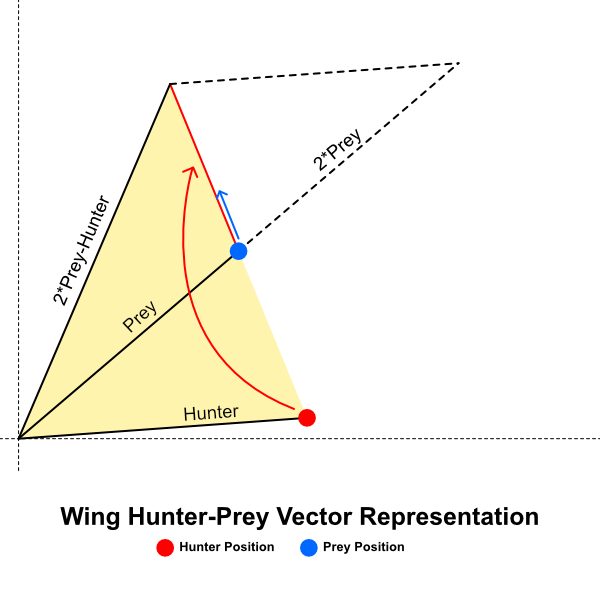
\includegraphics[width=0.65\textwidth]{img/pa/wing-hunt}
  \caption{Wing Hunt Vector Visualization}
  \end{center}
  \end{figure}
\end{frame}
\begin{frame}{Proposed Algorithm:Hunting}
  \begin{figure}[h]
  \begin{center}
  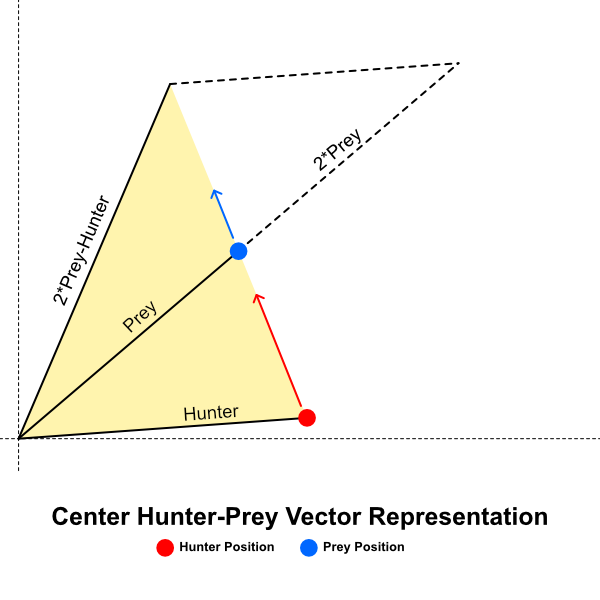
\includegraphics[width=0.65\textwidth]{img/pa/center-hunt}
  \caption{Center Hunt Vector Visualization}
  \end{center}
  \end{figure}
\end{frame}

\begin{frame}{Proposed Algorithm: Moving towards safe place}
As mentioned earlier, some of the females in a pride go hunting, not all.\\So, remaining females go toward one of the areas of the territory.\\This would improve the current solutions for the pride.\\Females would go toward other lions selected using tournament selection.
\end{frame}

\begin{frame}{Proposed Algorithm: Moving towards safe place}
  \begin{figure}[h]
  \begin{center}
  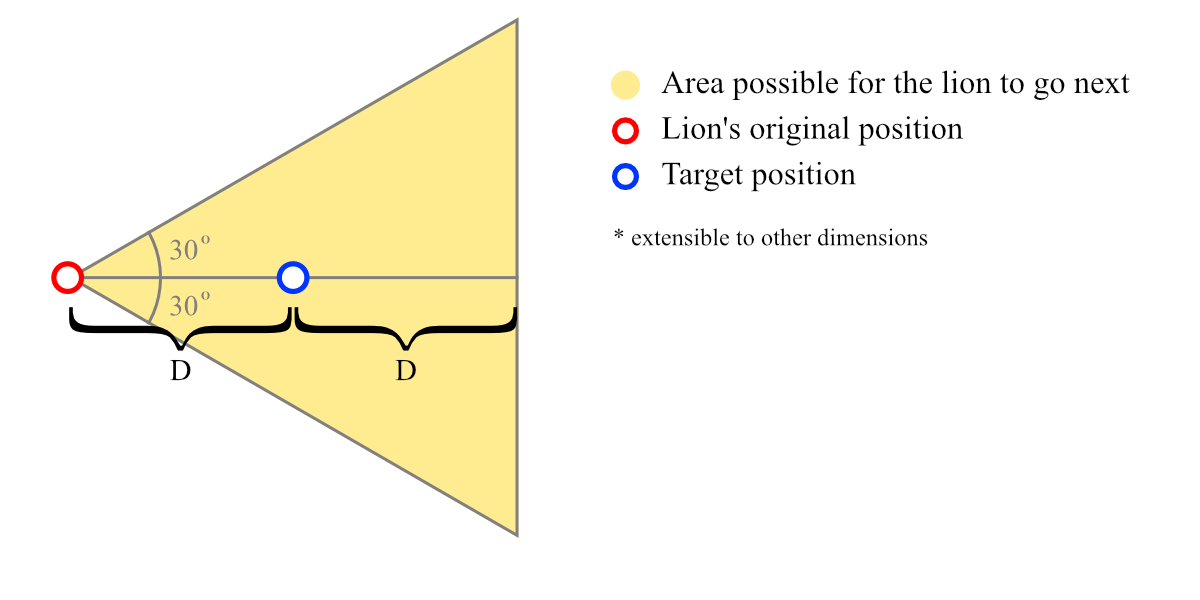
\includegraphics[width=0.65\textwidth]{img/moving/moving}
  \caption{Range of next positions relative to original}
  \end{center}
  \end{figure}
\end{frame}

\begin{frame}{Proposed Algorithm: Roaming}
Male lions in a pride would also roam in their territory.\\Male lions use the same mechanism in the previous section but using random selection instead.
\end{frame}

\begin{frame}{Proposed Algorithm: Roaming}
Nomad lions, unlike residents, roam sporadically.\\Nomad positions are randomly generated but still saves the best position.\\These positions change more often when the lion is far from the best fit among the nomads.
\end{frame}

\begin{frame}{Proposed Algorithm: Mating}
%--dito
\end{frame}

\begin{frame}{Proposed Algorithm: Defense}
%--dito
\end{frame}

\begin{frame}{Proposed Algorithm: Migration}
%--dito
\end{frame}

\begin{frame}{Proposed Algorithm: Equilibrium}
%--dito
\end{frame}

\begin{frame}{Sample Runs and Benchmarks}
The algorithm is now tested upon different benchmarking functions. There are 8 used functions to test the effectiveness of the algorithm, 4 of which are used again run in another solution space.
\end{frame}
\begin{frame}{Parabola}
$$
  g1=f(x) = x^2
$$
\end{frame}
\begin{frame}{Parabola}
  \begin{figure}[h]
  \begin{center}
    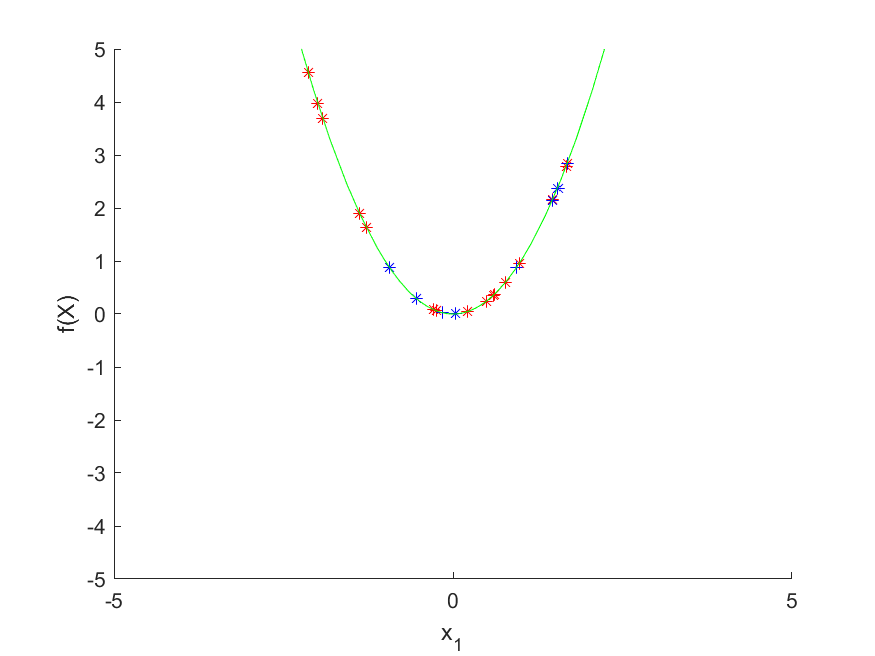
\includegraphics[width=0.65\textwidth]{img/smpl/circ/loa-iter-0}
    \caption{Iteration 0}
  \end{center}
  \end{figure}
\end{frame}
\begin{frame}{Parabola}
  \begin{figure}[h]
  \begin{center}
    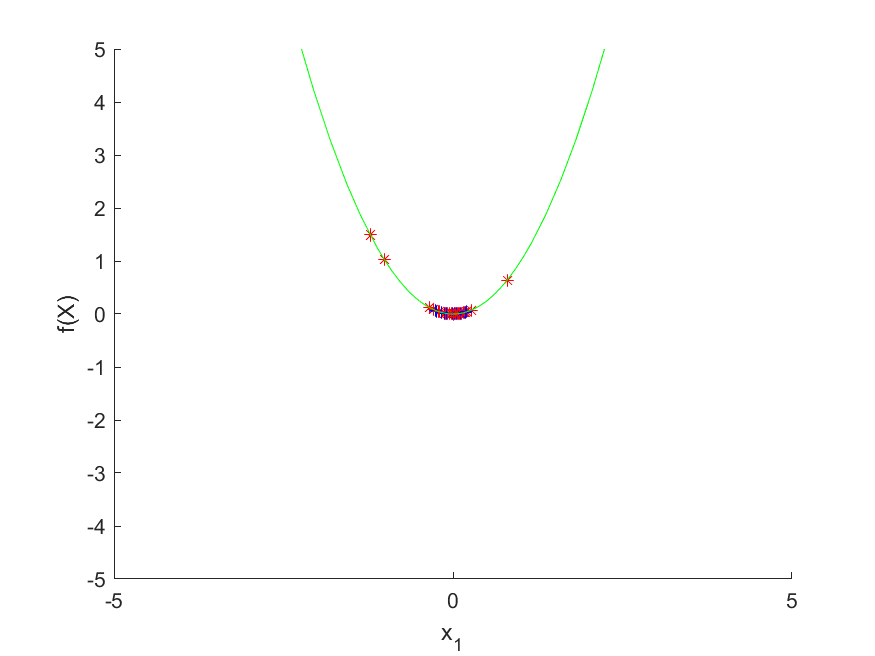
\includegraphics[width=0.65\textwidth]{img/smpl/circ/loa-iter-7}
    \caption{Iteration 7}
  \end{center}
  \end{figure}
\end{frame}
\begin{frame}{Parabola}
  \begin{figure}[h]
  \begin{center}
    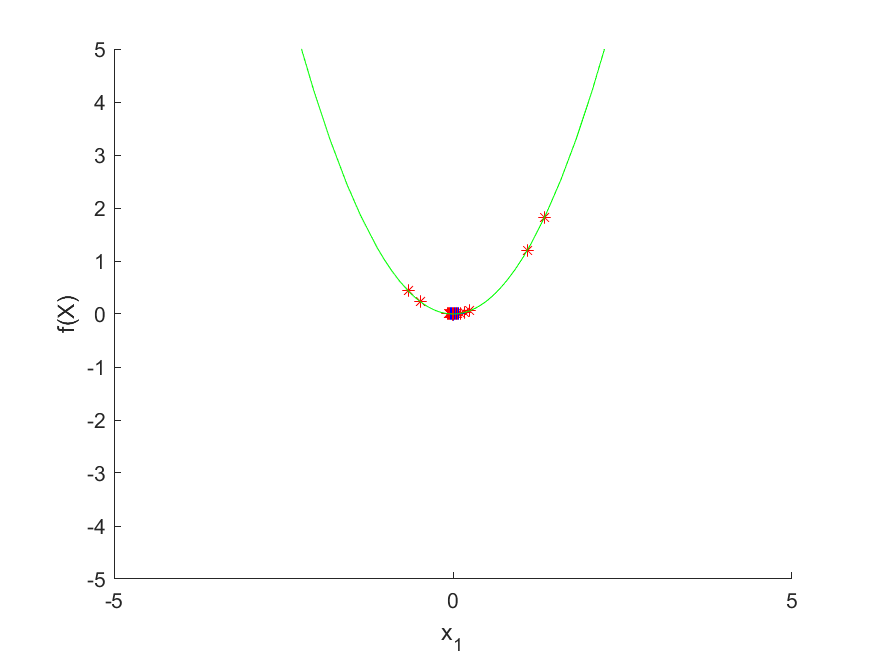
\includegraphics[width=0.65\textwidth]{img/smpl/circ/loa-iter-14}
    \caption{Iteration 14}
  \end{center}
  \end{figure}
\end{frame}
\begin{frame}{Parabola}
  \begin{figure}[h]
  \begin{center}
    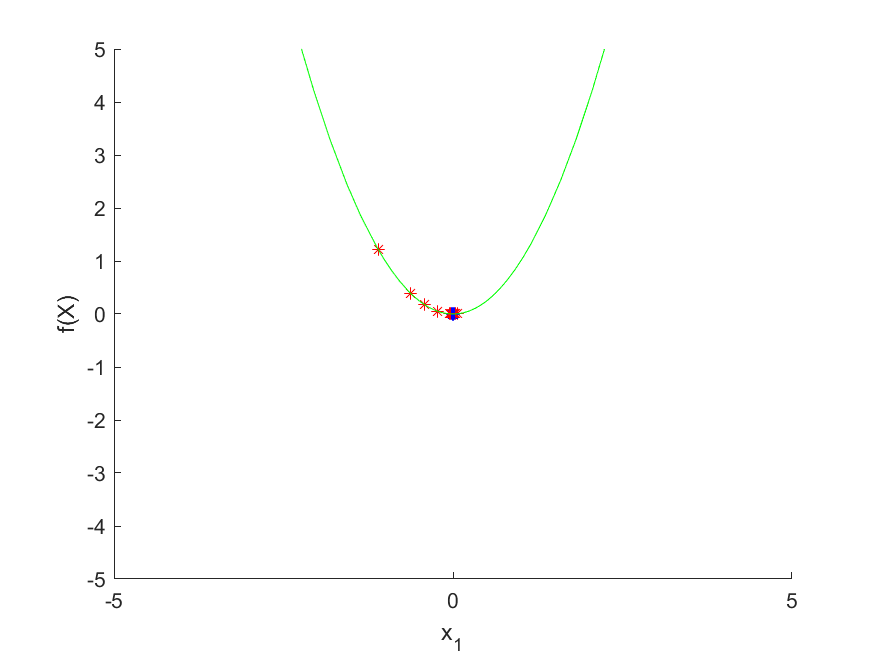
\includegraphics[width=0.65\textwidth]{img/smpl/circ/loa-iter-21}
    \caption{Iteration 21}
  \end{center}
  \end{figure}
\end{frame}
\begin{frame}{Parabola}
  \begin{figure}[h]
  \begin{center}
    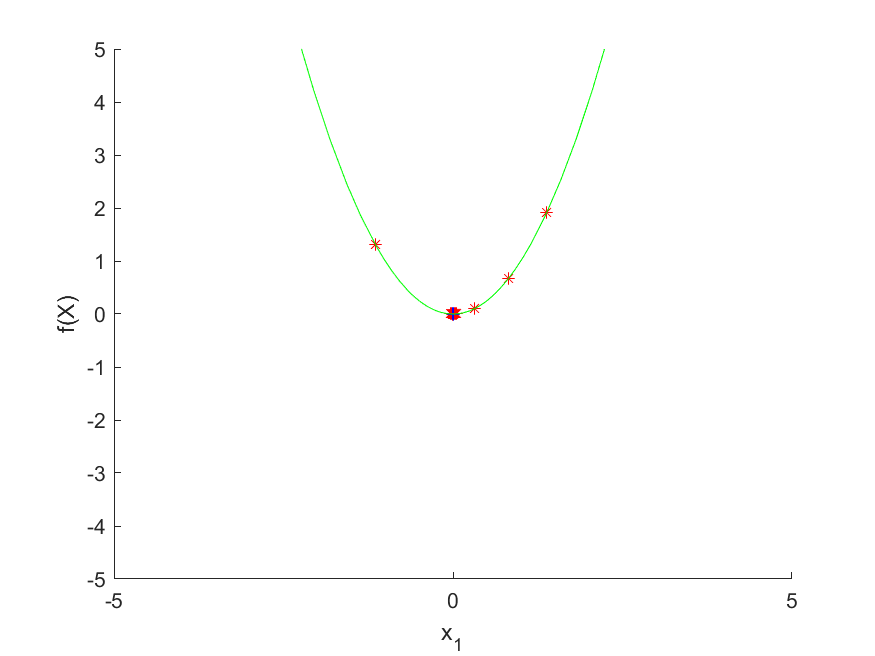
\includegraphics[width=0.65\textwidth]{img/smpl/circ/loa-iter-28}
    \caption{Iteration 28}
  \end{center}
  \end{figure}
\end{frame}
\begin{frame}{Parabola}
  \begin{figure}[h]
  \begin{center}
    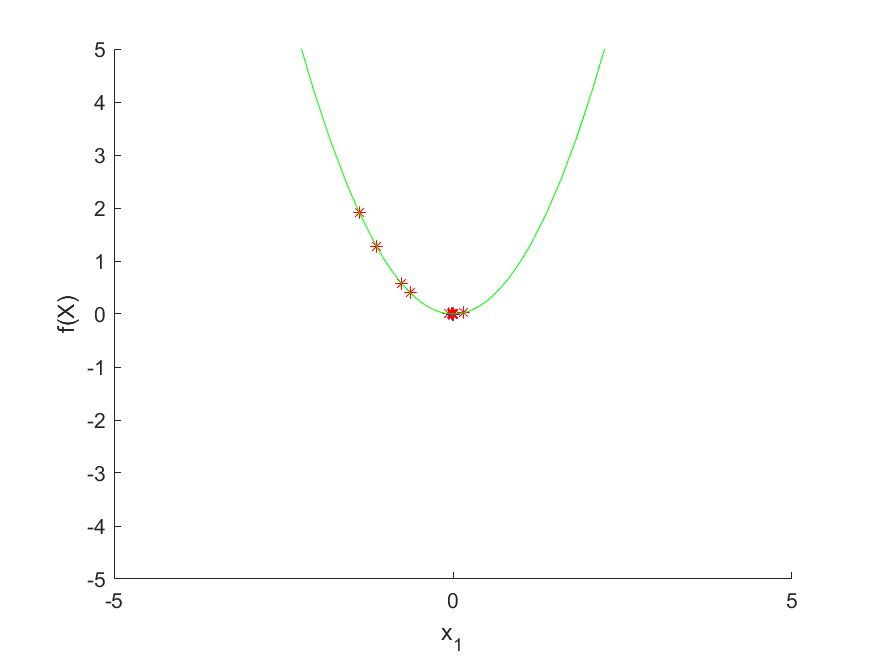
\includegraphics[width=0.65\textwidth]{img/smpl/circ/loa-iter-35}
    \caption{Iteration 35}
  \end{center}
  \end{figure}
\end{frame}
\begin{frame}{Parabola}
  \begin{figure}[h]
  \begin{center}
    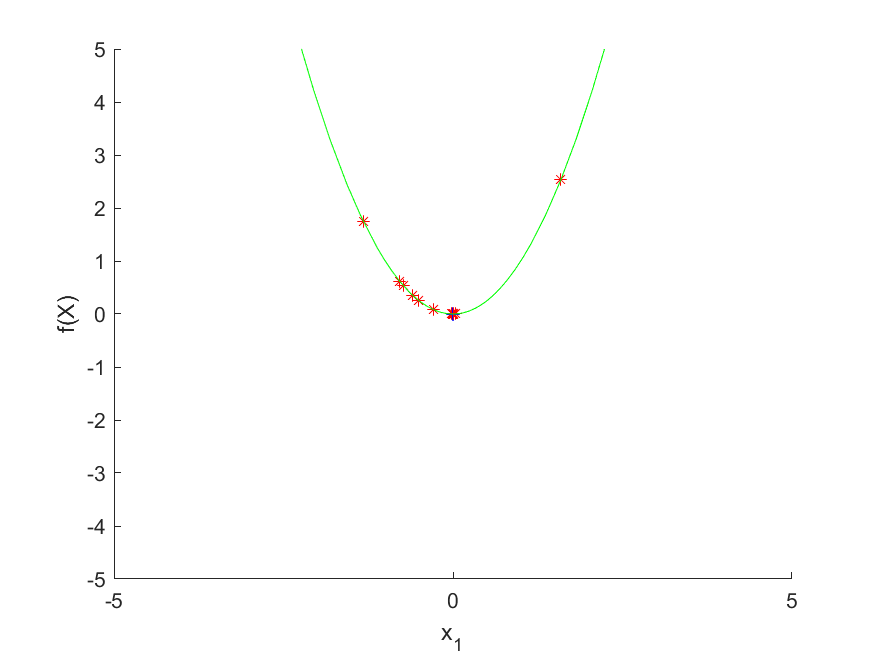
\includegraphics[width=0.65\textwidth]{img/smpl/circ/loa-iter-42}
    \caption{Iteration 42}
  \end{center}
  \end{figure}
\end{frame}
\begin{frame}{Parabola}
  \begin{figure}[h]
  \begin{center}
    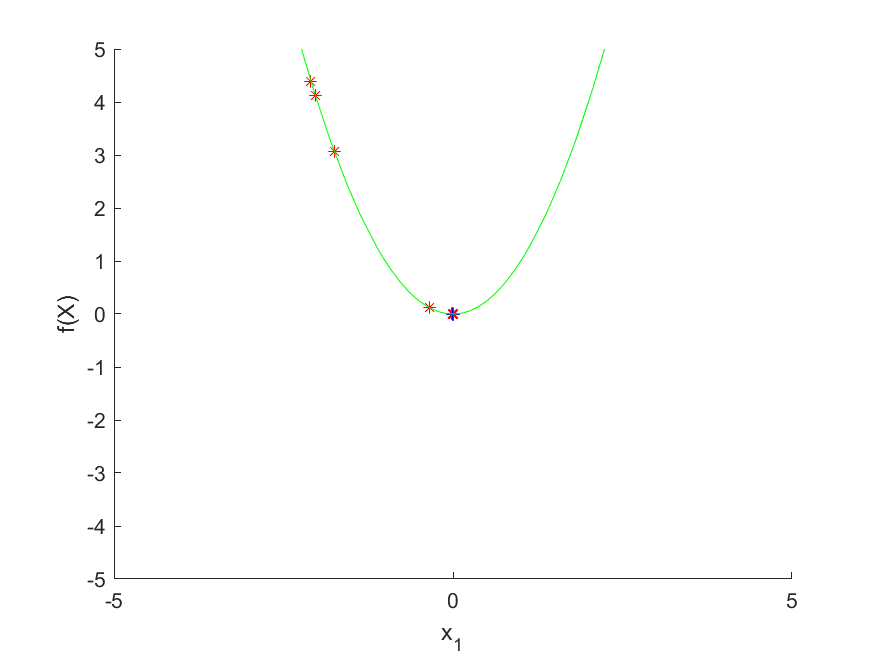
\includegraphics[width=0.65\textwidth]{img/smpl/circ/loa-iter-50}
    \caption{Iteration 50}
  \end{center}
  \end{figure}
\end{frame}

\begin{frame}{Rastrigin 1D}
  $$
    g3=f(x) = 10 + x^2 - 10 \cos(2\pi x)
  $$
\end{frame}
\begin{frame}{Rastrigin 1D}
  \begin{figure}[h]
  \begin{center}
    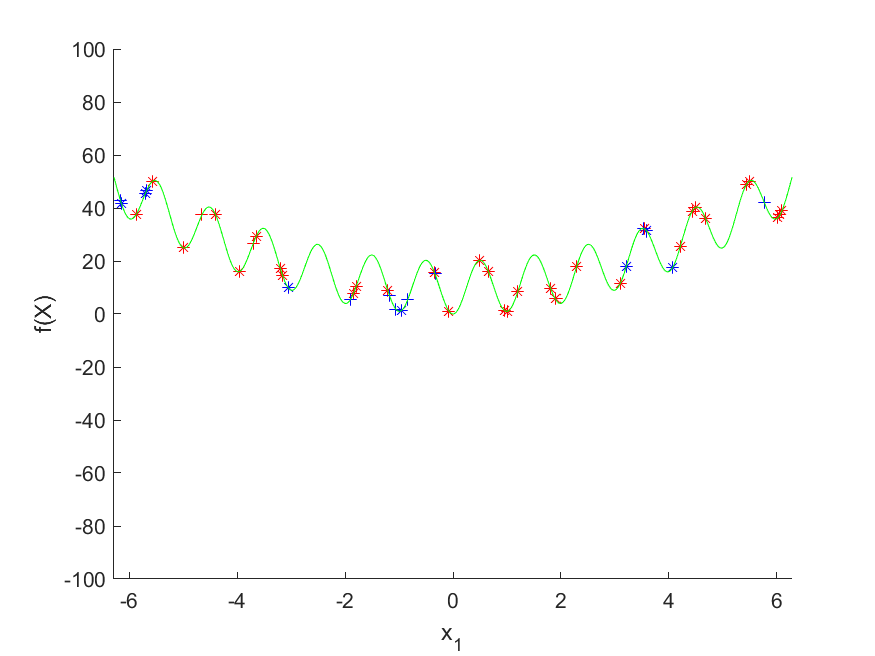
\includegraphics[width=0.65\textwidth]{img/smpl/rast1d/loa-iter-0}
    \caption{Iteration 0}
  \end{center}
  \end{figure}
\end{frame}
\begin{frame}{Rastrigin 1D}
  \begin{figure}[h]
  \begin{center}
    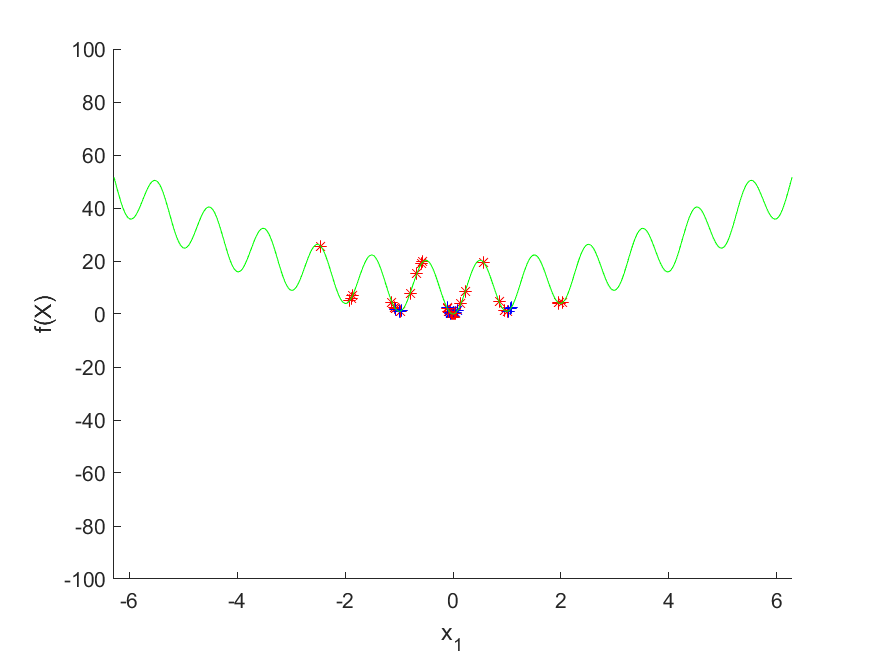
\includegraphics[width=0.65\textwidth]{img/smpl/rast1d/loa-iter-7}
    \caption{Iteration 7}
  \end{center}
  \end{figure}
\end{frame}
\begin{frame}{Rastrigin 1D}
  \begin{figure}[h]
  \begin{center}
    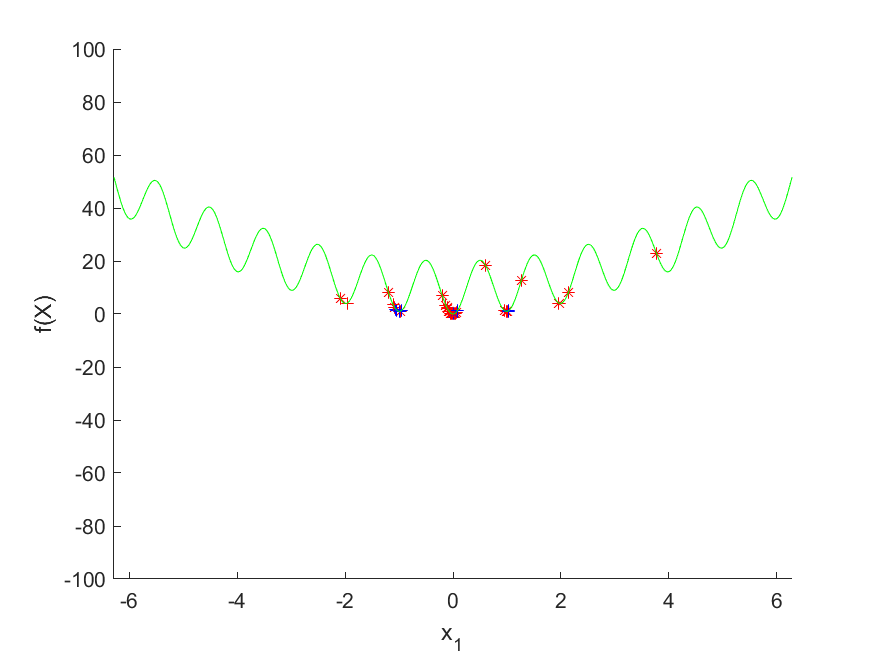
\includegraphics[width=0.65\textwidth]{img/smpl/rast1d/loa-iter-14}
    \caption{Iteration 14}
  \end{center}
  \end{figure}
\end{frame}
\begin{frame}{Rastrigin 1D}
  \begin{figure}[h]
  \begin{center}
    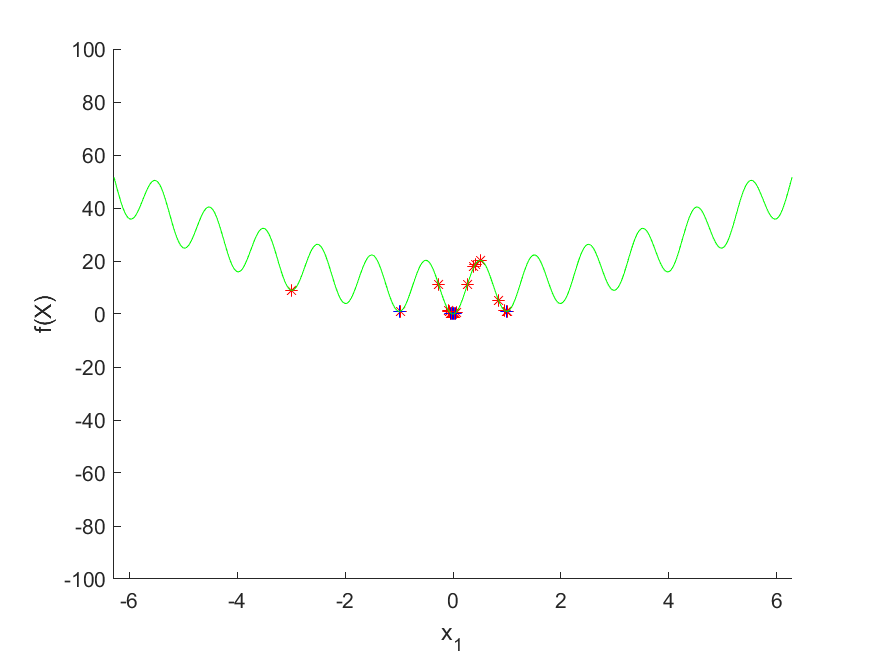
\includegraphics[width=0.65\textwidth]{img/smpl/rast1d/loa-iter-21}
    \caption{Iteration 21}
  \end{center}
  \end{figure}
\end{frame}
\begin{frame}{Rastrigin 1D}
  \begin{figure}[h]
  \begin{center}
    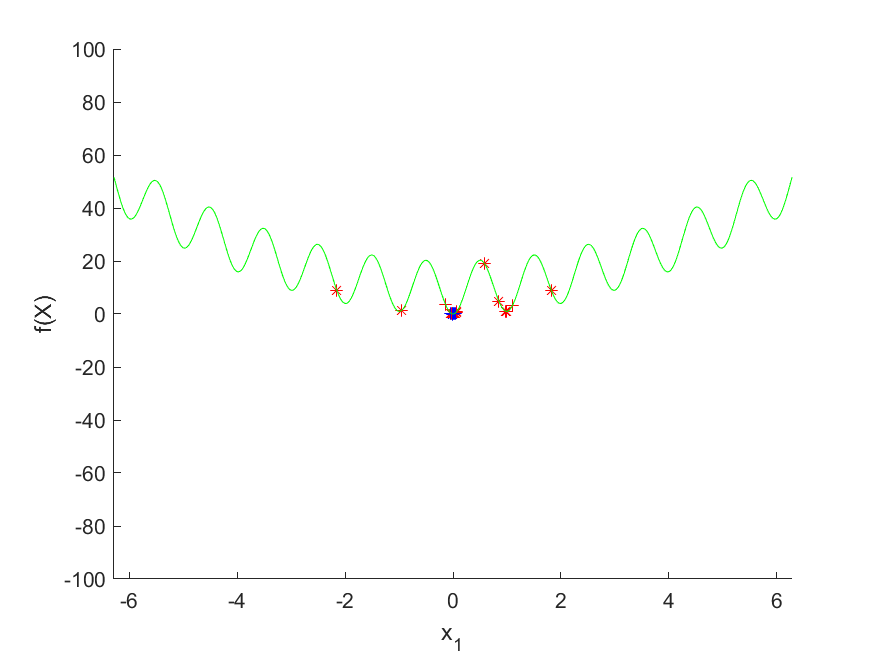
\includegraphics[width=0.65\textwidth]{img/smpl/rast1d/loa-iter-28}
    \caption{Iteration 28}
  \end{center}
  \end{figure}
\end{frame}
\begin{frame}{Rastrigin 1D}
  \begin{figure}[h]
  \begin{center}
    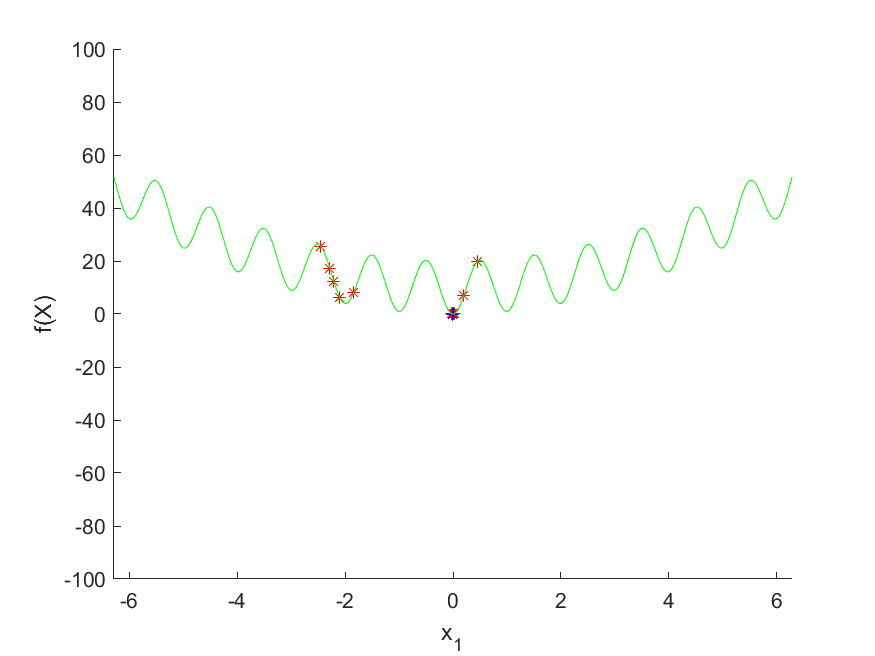
\includegraphics[width=0.65\textwidth]{img/smpl/rast1d/loa-iter-35}
    \caption{Iteration 35}
  \end{center}
  \end{figure}
\end{frame}
\begin{frame}{Rastrigin 1D}
  \begin{figure}[h]
  \begin{center}
    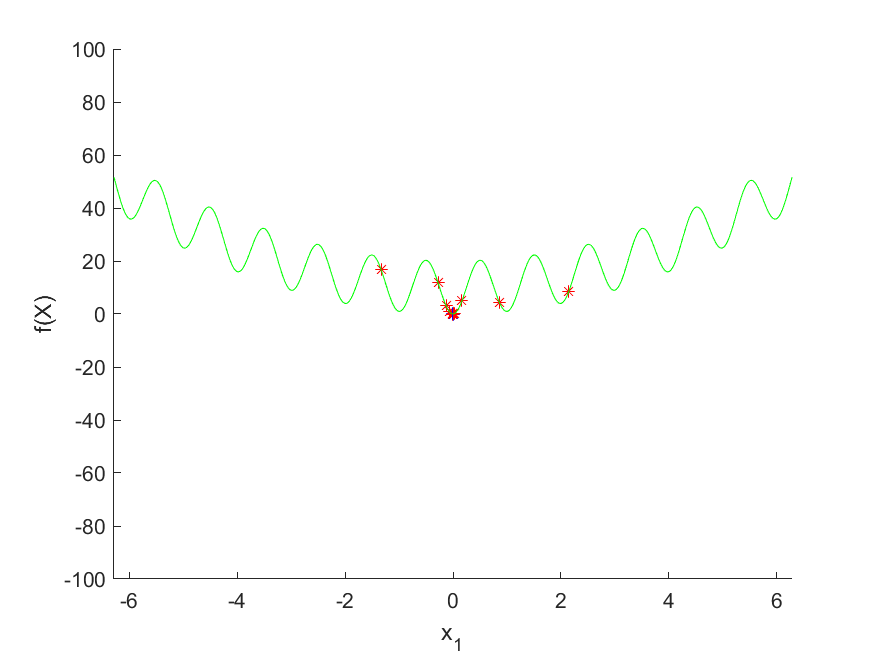
\includegraphics[width=0.65\textwidth]{img/smpl/rast1d/loa-iter-42}
    \caption{Iteration 42}
  \end{center}
  \end{figure}
\end{frame}
\begin{frame}{Rastrigin 1D}
  \begin{figure}[h]
  \begin{center}
    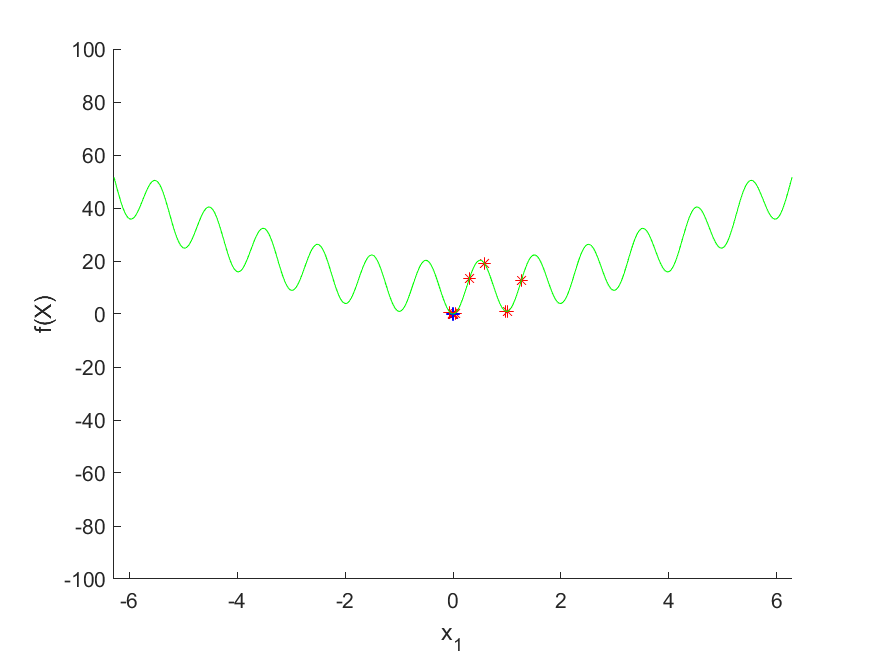
\includegraphics[width=0.65\textwidth]{img/smpl/rast1d/loa-iter-50}
    \caption{Iteration 50}
  \end{center}
  \end{figure}
\end{frame}

\begin{frame}{Rastrigin 2D}
  $$
   g4= f(x_1, x_2) = 20 + x_1^2 - 10 \cos(2\pi x_1) + x_2^2 - 10 \cos(2\pi x_2)
  $$
\end{frame}
\begin{frame}{Rastrigin 2D}
  \begin{figure}[h]
  \begin{center}
    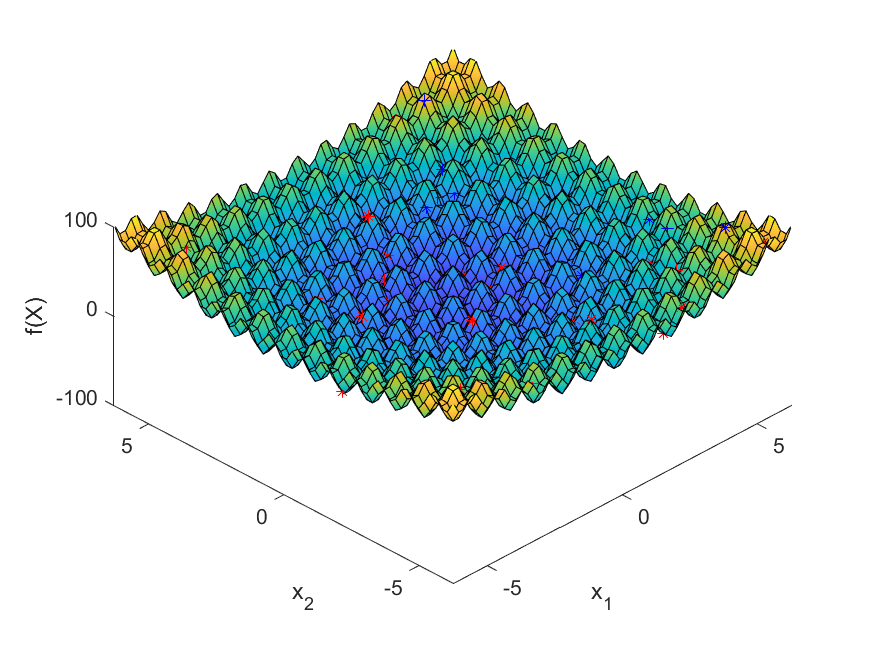
\includegraphics[width=0.65\textwidth]{img/smpl/rast2d/loa-iter-0}
    \caption{Iteration 0}
  \end{center}
  \end{figure}
\end{frame}
\begin{frame}{Rastrigin 2D}
  \begin{figure}[h]
  \begin{center}
    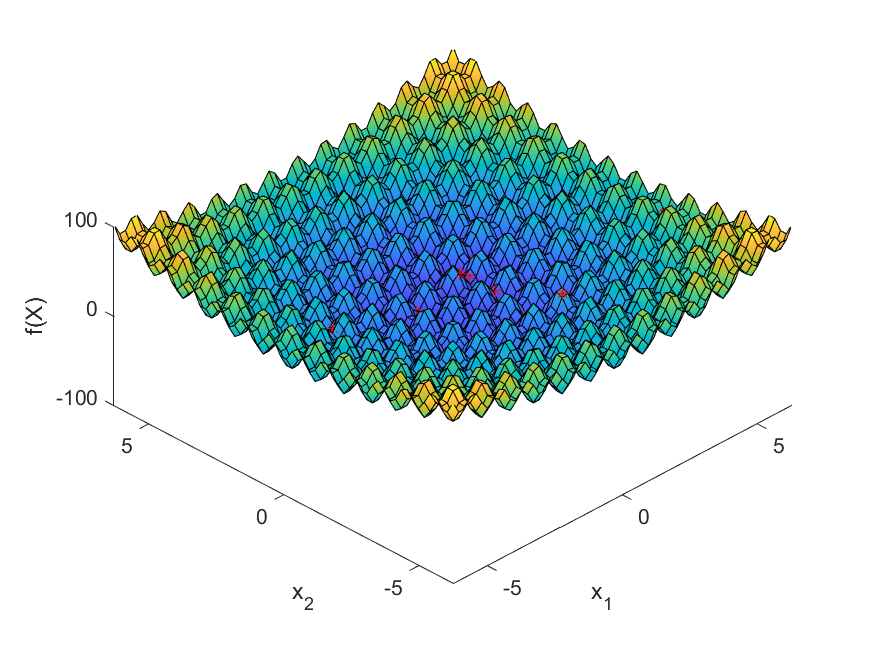
\includegraphics[width=0.65\textwidth]{img/smpl/rast2d/loa-iter-7}
    \caption{Iteration 7}
  \end{center}
  \end{figure}
\end{frame}
\begin{frame}{Rastrigin 2D}
  \begin{figure}[h]
  \begin{center}
    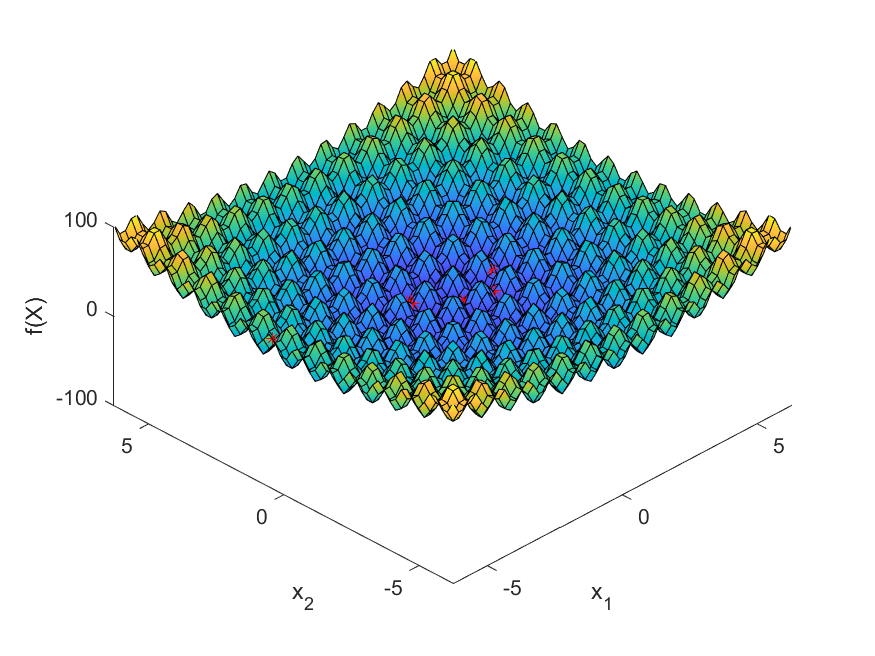
\includegraphics[width=0.65\textwidth]{img/smpl/rast2d/loa-iter-14}
    \caption{Iteration 14}
  \end{center}
  \end{figure}
\end{frame}
\begin{frame}{Rastrigin 2D}
  \begin{figure}[h]
  \begin{center}
    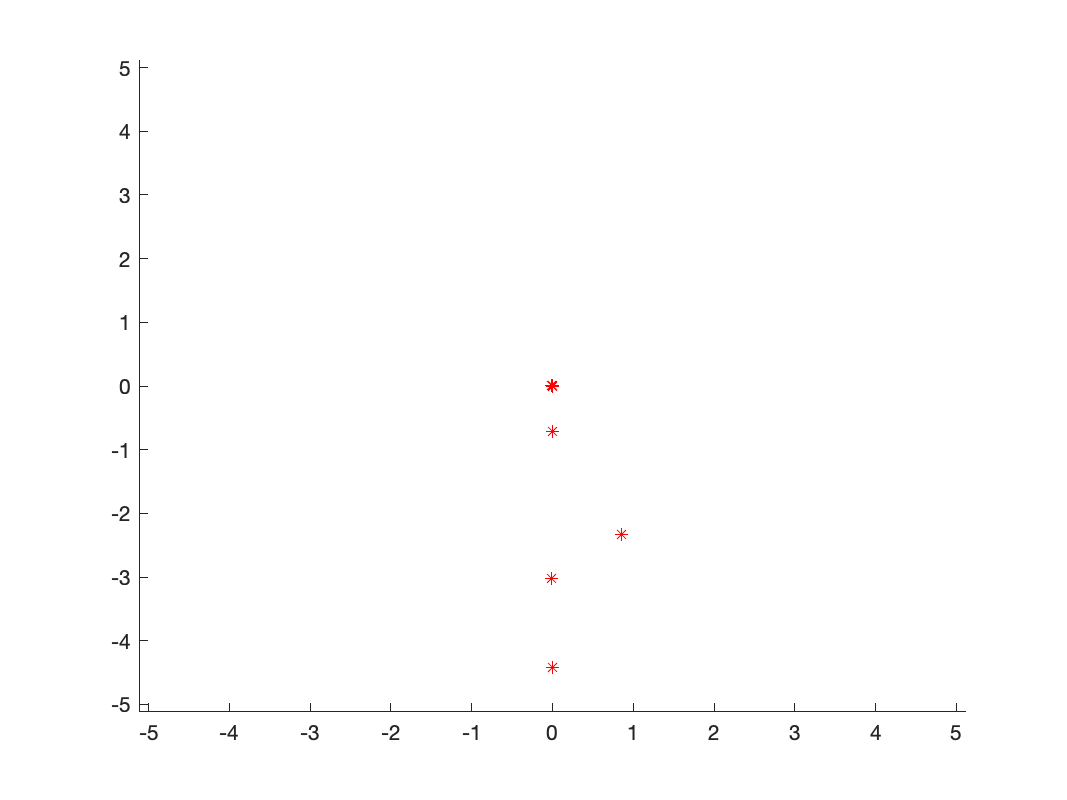
\includegraphics[width=0.65\textwidth]{img/smpl/rast2d/loa-iter-21}
    \caption{Iteration 21}
  \end{center}
  \end{figure}
\end{frame}
\begin{frame}{Rastrigin 2D}
  \begin{figure}[h]
  \begin{center}
    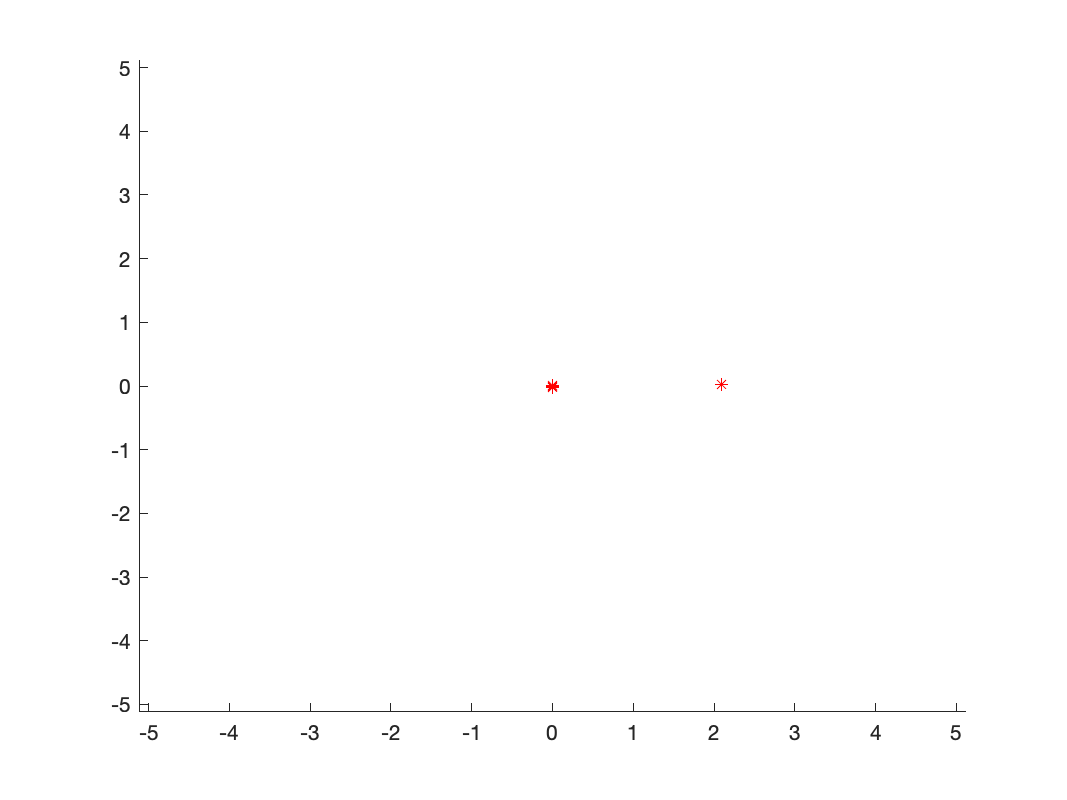
\includegraphics[width=0.65\textwidth]{img/smpl/rast2d/loa-iter-28}
    \caption{Iteration 28}
  \end{center}
  \end{figure}
\end{frame}
\begin{frame}{Rastrigin 2D}
  \begin{figure}[h]
  \begin{center}
    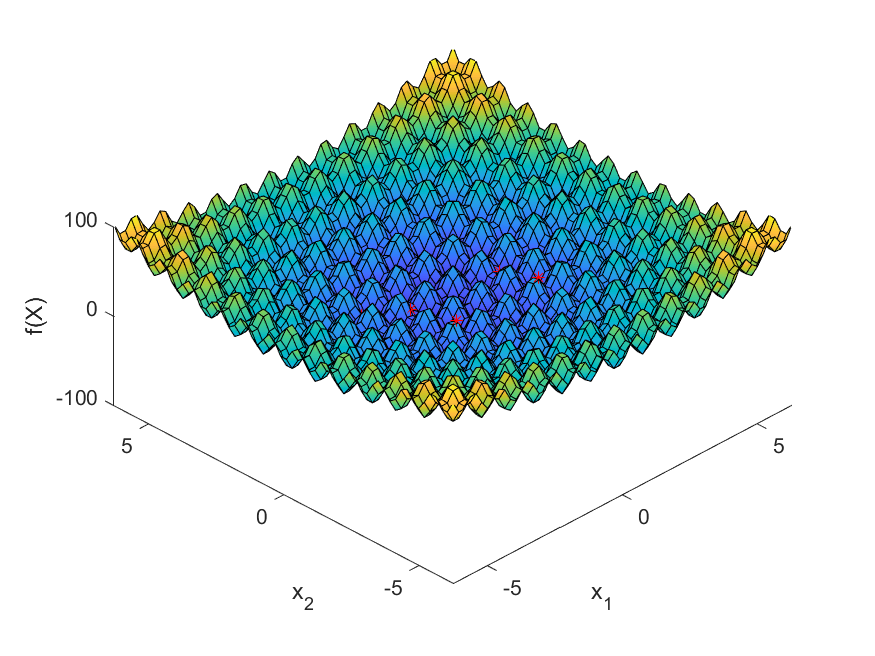
\includegraphics[width=0.65\textwidth]{img/smpl/rast2d/loa-iter-35}
    \caption{Iteration 35}
  \end{center}
  \end{figure}
\end{frame}
\begin{frame}{Rastrigin 2D}
  \begin{figure}[h]
  \begin{center}
    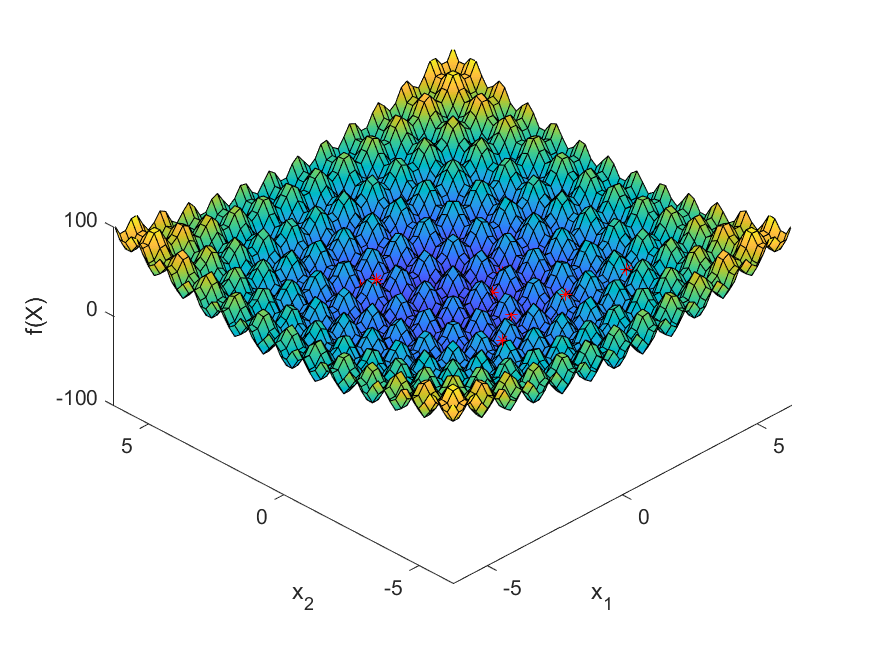
\includegraphics[width=0.65\textwidth]{img/smpl/rast2d/loa-iter-42}
    \caption{Iteration 42}
  \end{center}
  \end{figure}
\end{frame}
\begin{frame}{Rastrigin 2D}
  \begin{figure}[h]
  \begin{center}
    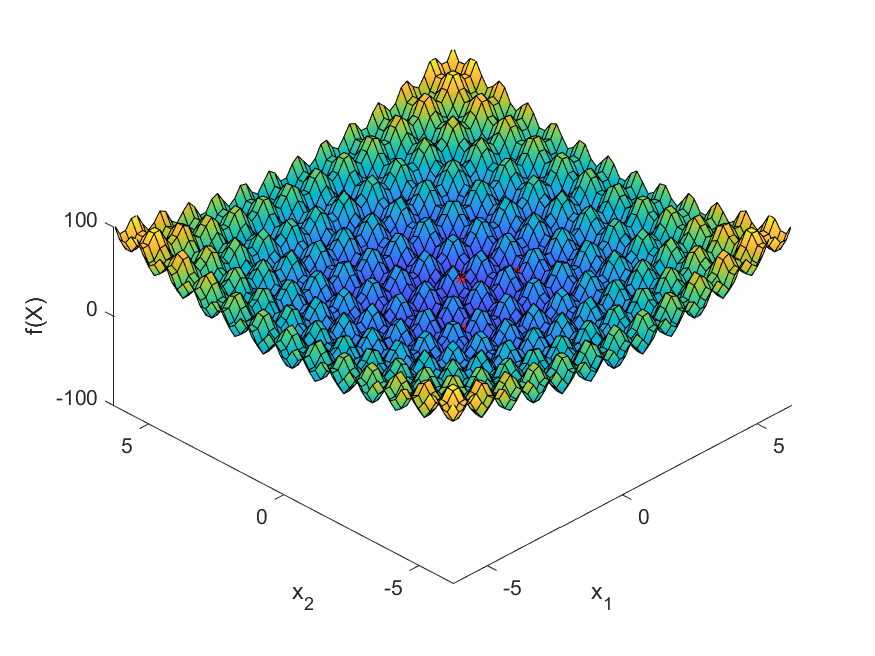
\includegraphics[width=0.65\textwidth]{img/smpl/rast2d/loa-iter-50}
    \caption{Iteration 50}
  \end{center}
  \end{figure}
\end{frame}

\begin{frame}{Rosenbrock 2D}
  $$
    g5=f(x_1, x_2) = (a-x_1)^2+b(x_2-x_1^2)^2
  $$
  with $a = 1$ and $b=100$. It has a global minimum at $(x_1, x_2) = (a, a^2)$.
\end{frame}
\begin{frame}{Rosenbrock 2D}
  \begin{figure}[h]
  \begin{center}
    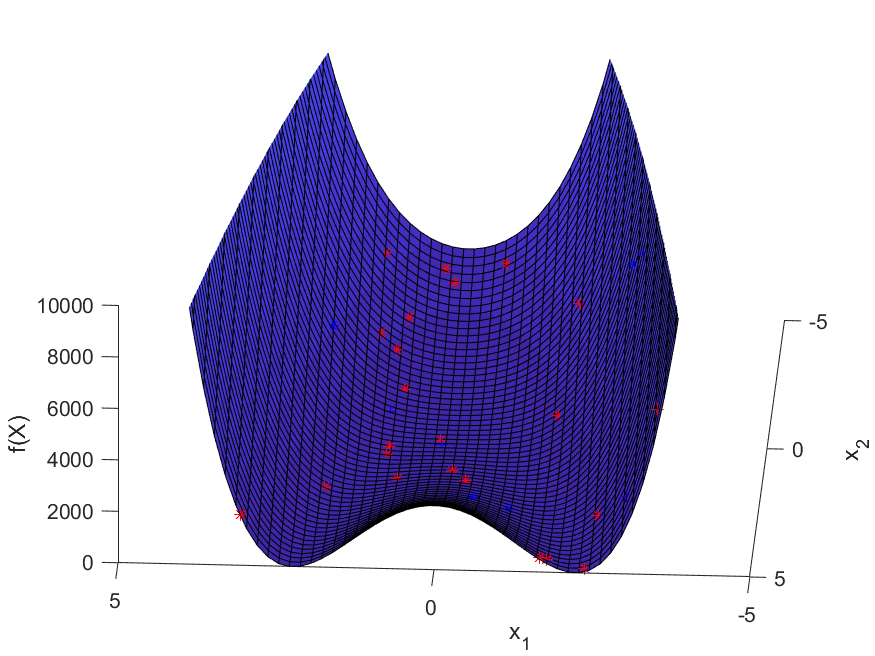
\includegraphics[width=0.65\textwidth]{img/smpl/rosn2d-1-100/loa-iter-0}
    \caption{Iteration 0}
  \end{center}
  \end{figure}
\end{frame}
\begin{frame}{Rosenbrock 2D}
  \begin{figure}[h]
  \begin{center}
    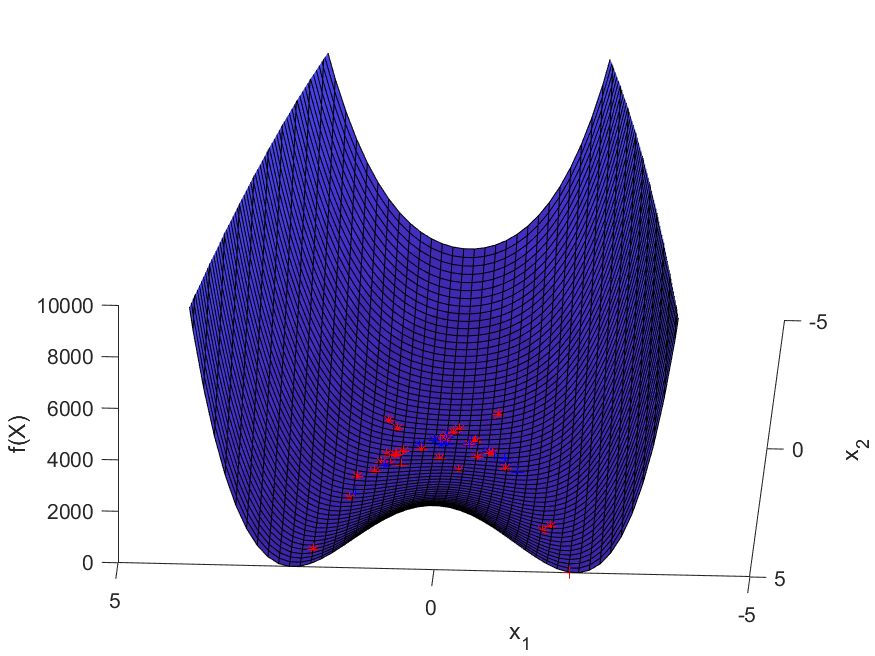
\includegraphics[width=0.65\textwidth]{img/smpl/rosn2d-1-100/loa-iter-7}
    \caption{Iteration 7}
  \end{center}
  \end{figure}
\end{frame}
\begin{frame}{Rosenbrock 2D}
  \begin{figure}[h]
  \begin{center}
    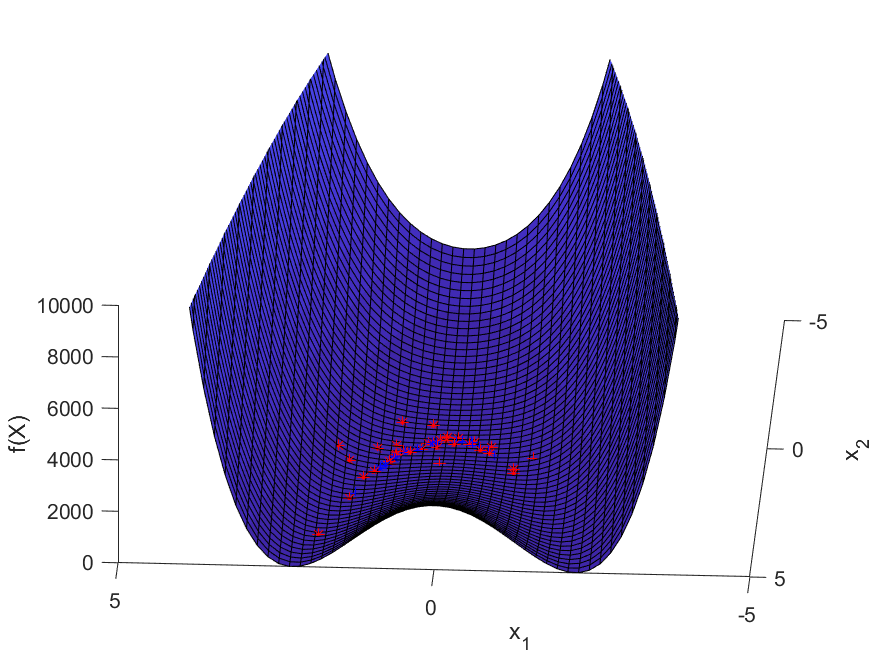
\includegraphics[width=0.65\textwidth]{img/smpl/rosn2d-1-100/loa-iter-14}
    \caption{Iteration 14}
  \end{center}
  \end{figure}
\end{frame}
\begin{frame}{Rosenbrock 2D}
  \begin{figure}[h]
  \begin{center}
    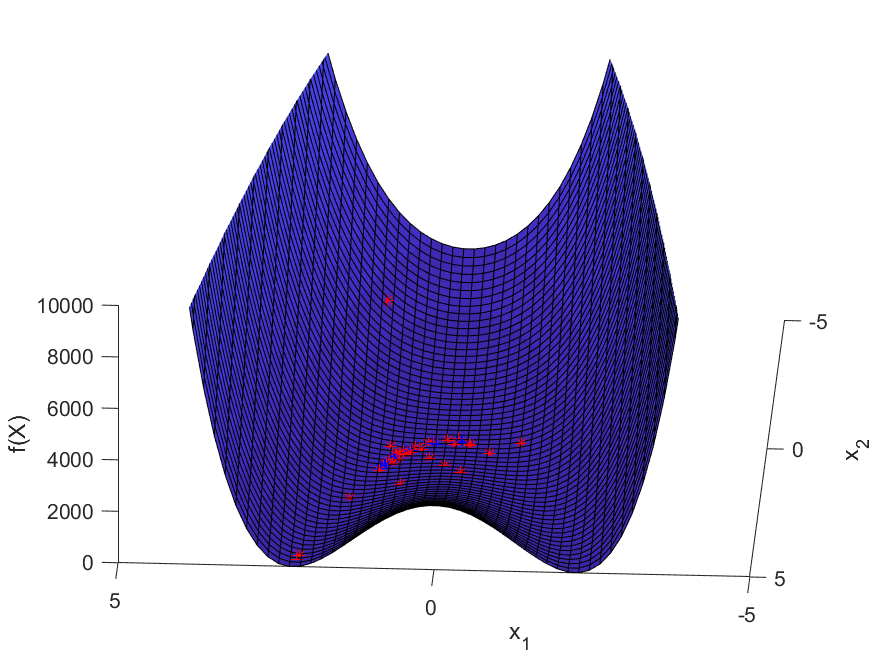
\includegraphics[width=0.65\textwidth]{img/smpl/rosn2d-1-100/loa-iter-21}
    \caption{Iteration 21}
  \end{center}
  \end{figure}
\end{frame}
\begin{frame}{Rosenbrock 2D}
  \begin{figure}[h]
  \begin{center}
    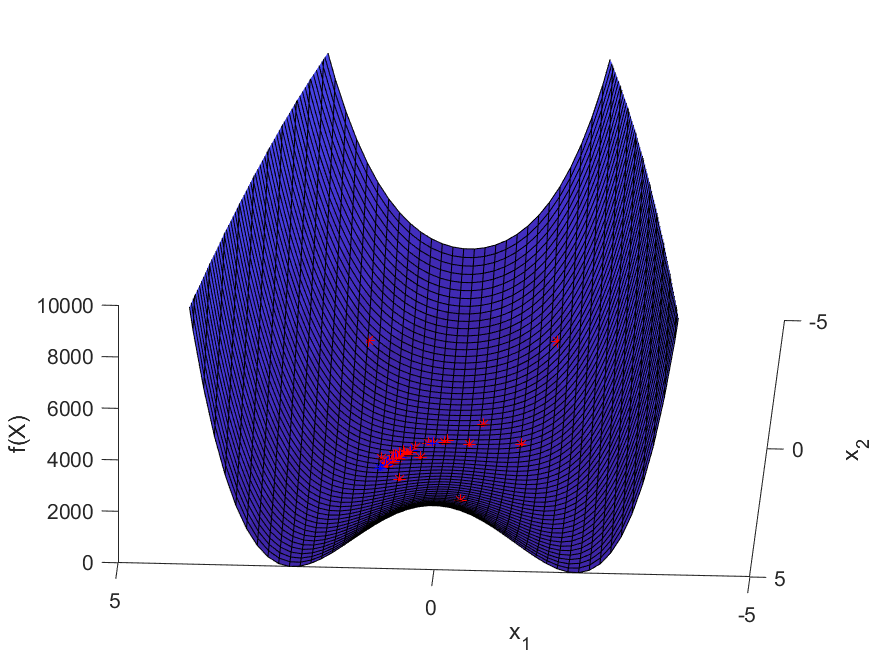
\includegraphics[width=0.65\textwidth]{img/smpl/rosn2d-1-100/loa-iter-28}
    \caption{Iteration 28}
  \end{center}
  \end{figure}
\end{frame}
\begin{frame}{Rosenbrock 2D}
  \begin{figure}[h]
  \begin{center}
    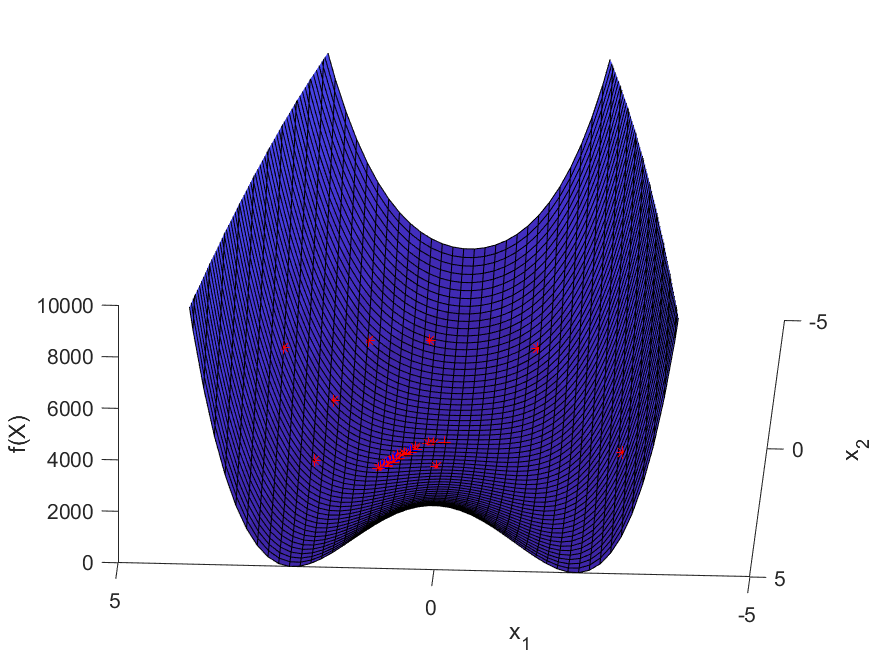
\includegraphics[width=0.65\textwidth]{img/smpl/rosn2d-1-100/loa-iter-35}
    \caption{Iteration 35}
  \end{center}
  \end{figure}
\end{frame}
\begin{frame}{Rosenbrock 2D}
  \begin{figure}[h]
  \begin{center}
    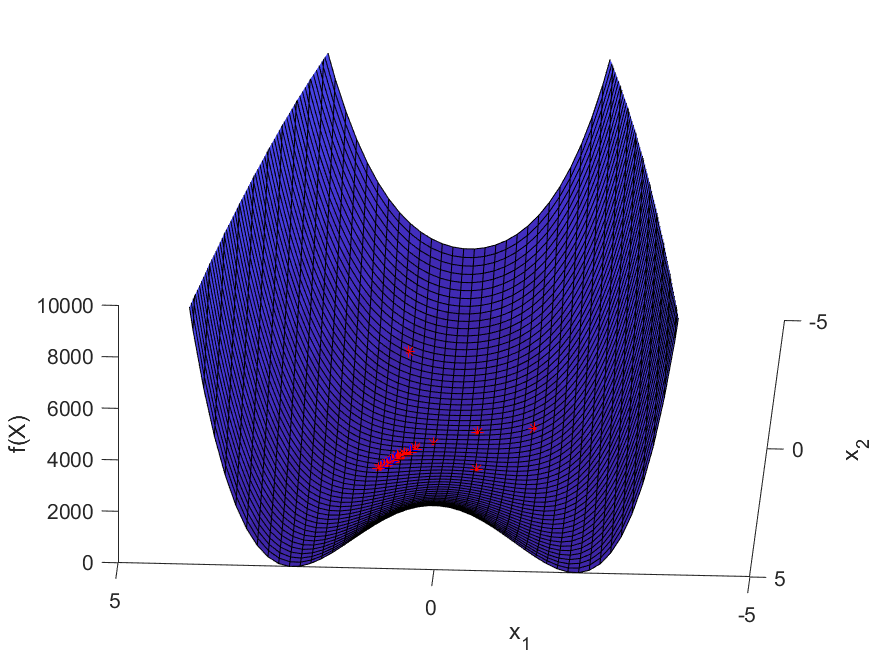
\includegraphics[width=0.65\textwidth]{img/smpl/rosn2d-1-100/loa-iter-42}
    \caption{Iteration 42}
  \end{center}
  \end{figure}
\end{frame}
\begin{frame}{Rosenbrock 2D}
  \begin{figure}[h]
  \begin{center}
    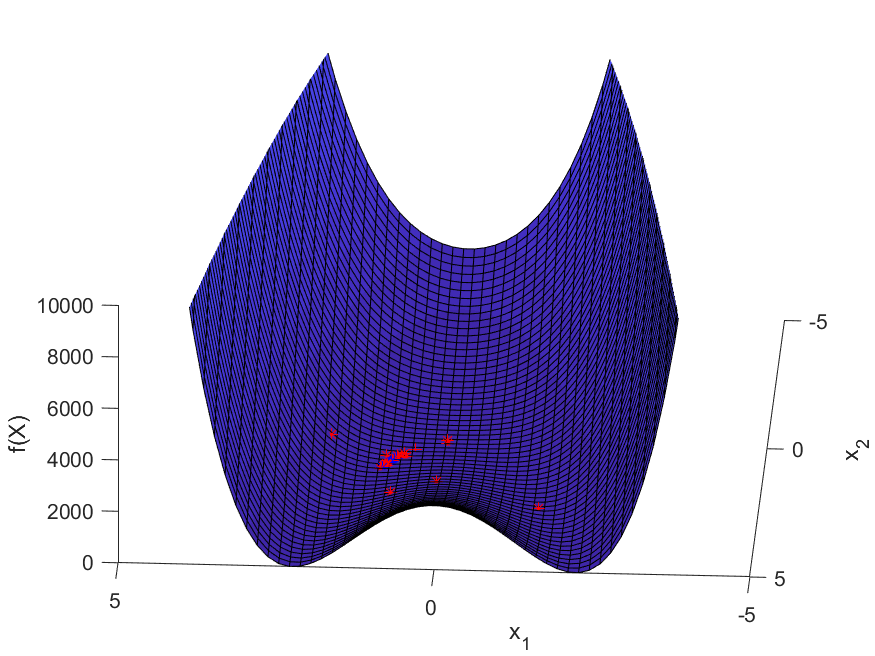
\includegraphics[width=0.65\textwidth]{img/smpl/rosn2d-1-100/loa-iter-50}
    \caption{Iteration 50}
  \end{center}
  \end{figure}
\end{frame}

\begin{frame}{Shifted Rastrigin 2D}
  The next test reuses Rastrigin 2D function ($g4$) in the interval of $x_i = [\pi, 2\pi]$.
\end{frame}
\begin{frame}{Shifted Rastrigin 2D}
  \begin{figure}[h]
  \begin{center}
    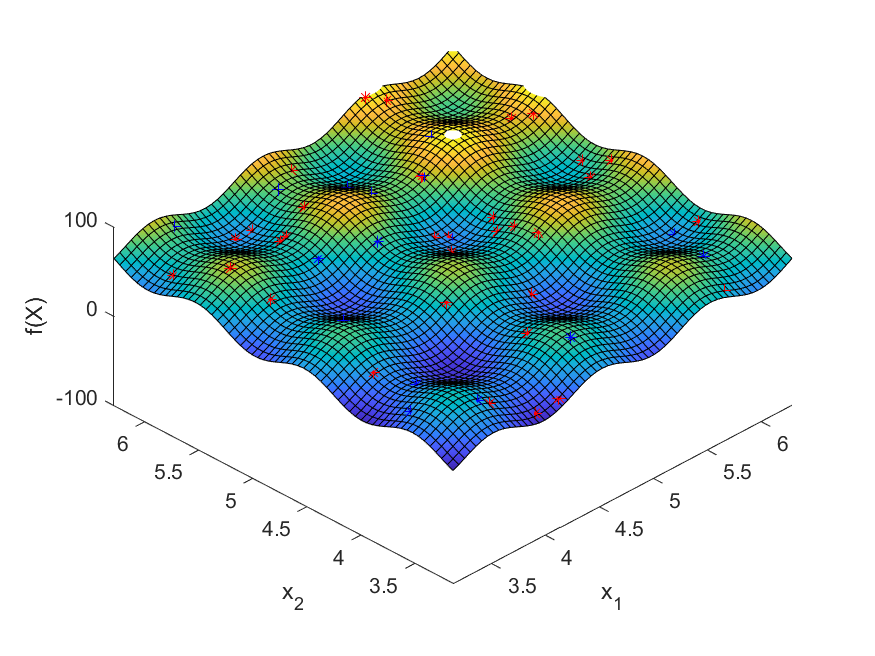
\includegraphics[width=0.65\textwidth]{img/smpl/rast2dshft/loa-iter-0}
    \caption{Iteration 0}
  \end{center}
  \end{figure}
\end{frame}
\begin{frame}{Shifted Rastrigin 2D}
  \begin{figure}[h]
  \begin{center}
    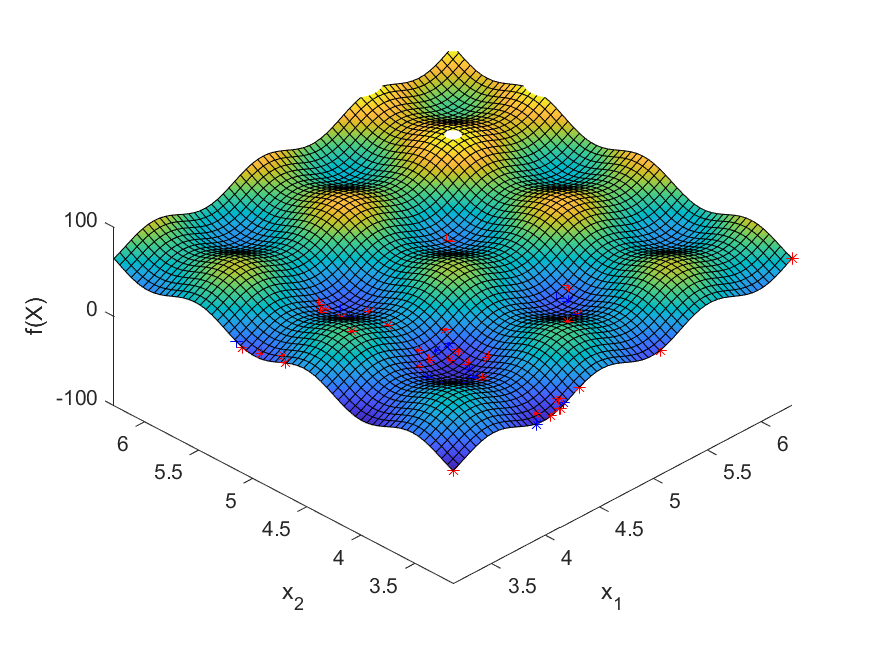
\includegraphics[width=0.65\textwidth]{img/smpl/rast2dshft/loa-iter-7}
    \caption{Iteration 7}
  \end{center}
  \end{figure}
\end{frame}
\begin{frame}{Shifted Rastrigin 2D}
  \begin{figure}[h]
  \begin{center}
    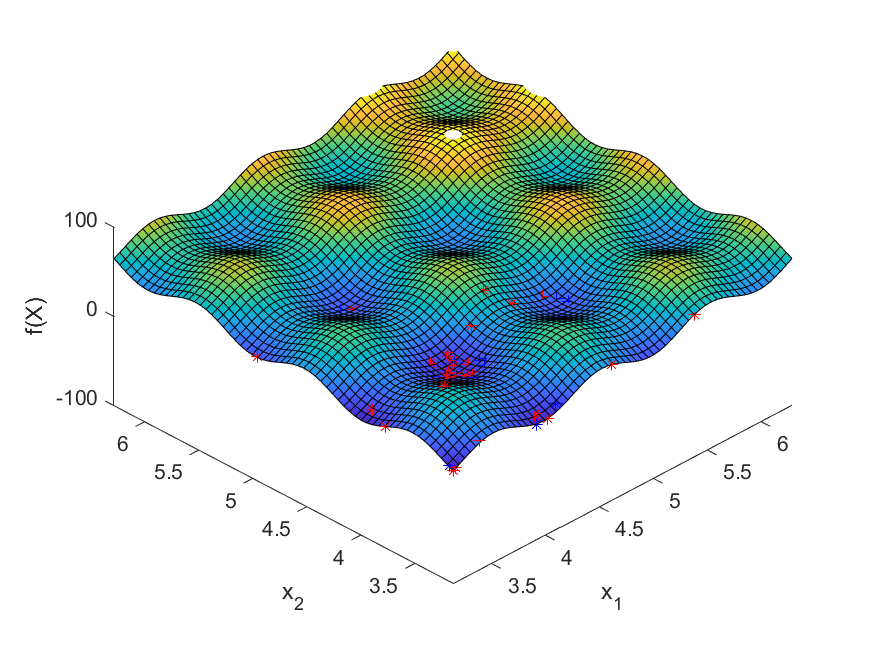
\includegraphics[width=0.65\textwidth]{img/smpl/rast2dshft/loa-iter-14}
    \caption{Iteration 14}
  \end{center}
  \end{figure}
\end{frame}
\begin{frame}{Shifted Rastrigin 2D}
  \begin{figure}[h]
  \begin{center}
    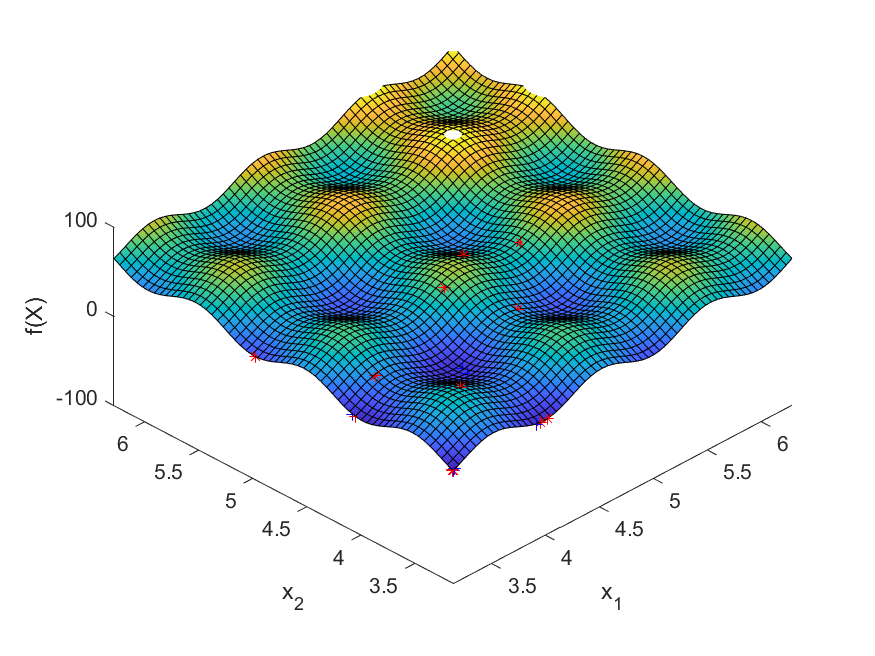
\includegraphics[width=0.65\textwidth]{img/smpl/rast2dshft/loa-iter-21}
    \caption{Iteration 21}
  \end{center}
  \end{figure}
\end{frame}
\begin{frame}{Shifted Rastrigin 2D}
  \begin{figure}[h]
  \begin{center}
    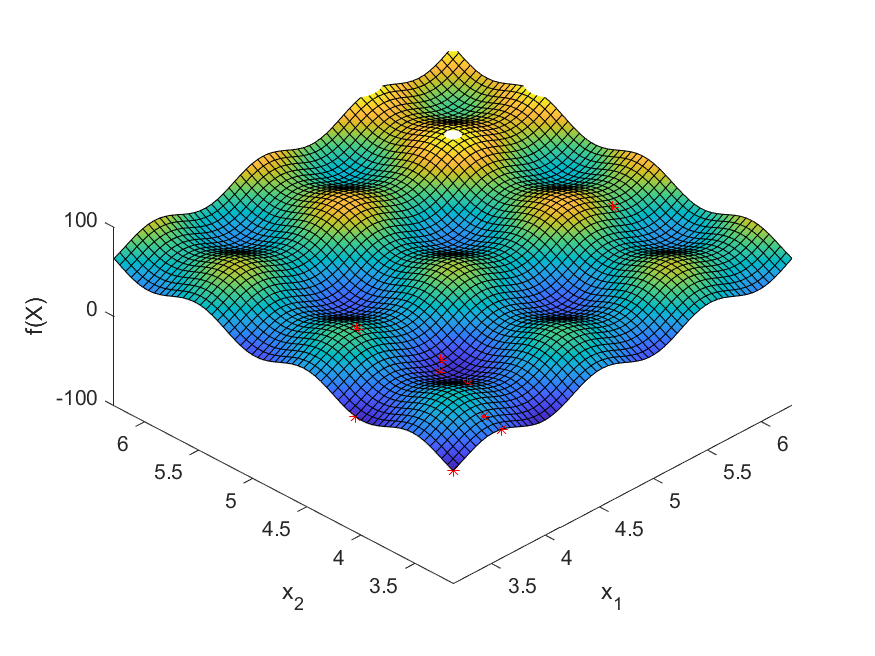
\includegraphics[width=0.65\textwidth]{img/smpl/rast2dshft/loa-iter-28}
    \caption{Iteration 28}
  \end{center}
  \end{figure}
\end{frame}
\begin{frame}{Shifted Rastrigin 2D}
  \begin{figure}[h]
  \begin{center}
    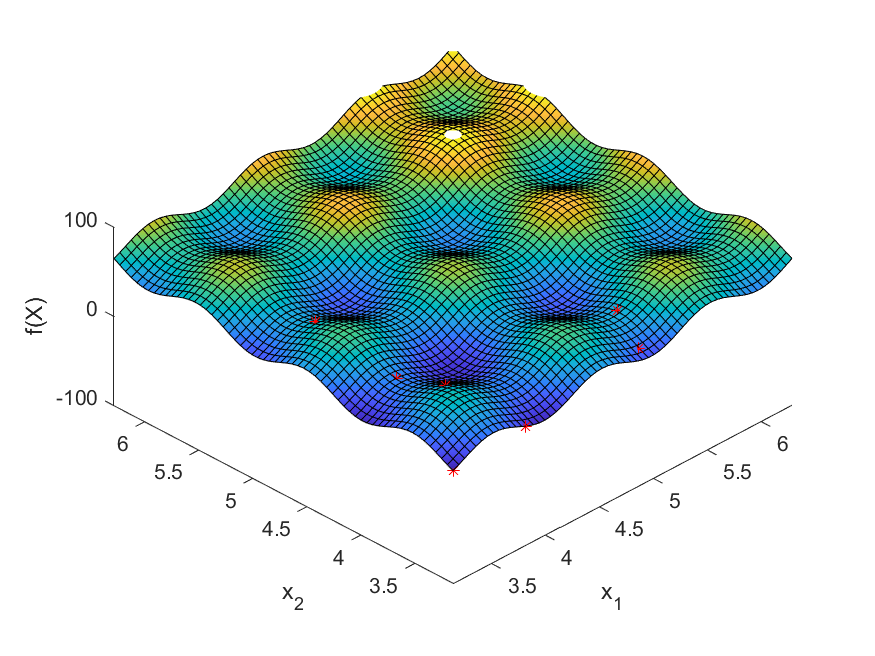
\includegraphics[width=0.65\textwidth]{img/smpl/rast2dshft/loa-iter-35}
    \caption{Iteration 35}
  \end{center}
  \end{figure}
\end{frame}
\begin{frame}{Shifted Rastrigin 2D}
  \begin{figure}[h]
  \begin{center}
    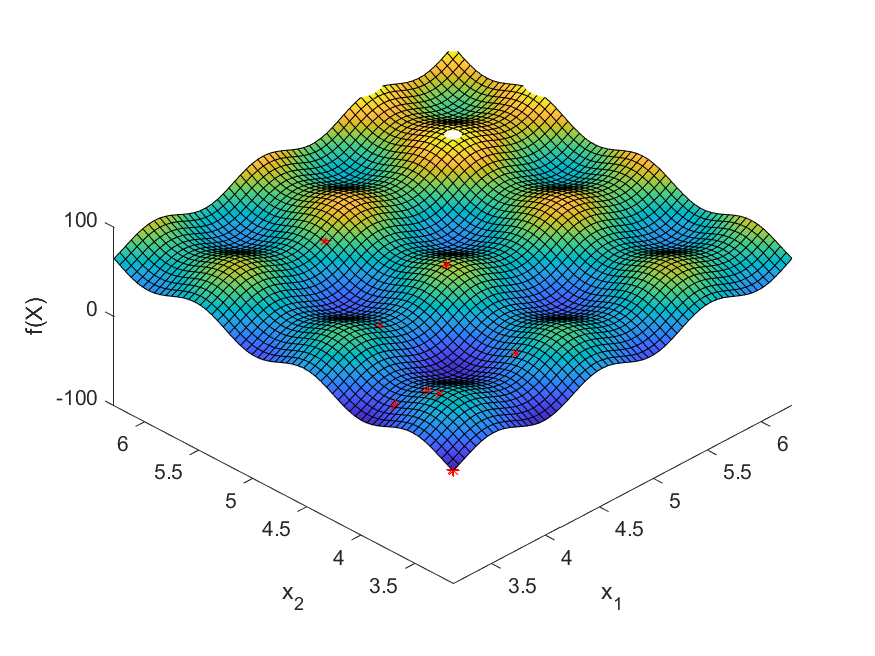
\includegraphics[width=0.65\textwidth]{img/smpl/rast2dshft/loa-iter-42}
    \caption{Iteration 42}
  \end{center}
  \end{figure}
\end{frame}
\begin{frame}{Shifted Rastrigin 2D}
  \begin{figure}[h]
  \begin{center}
    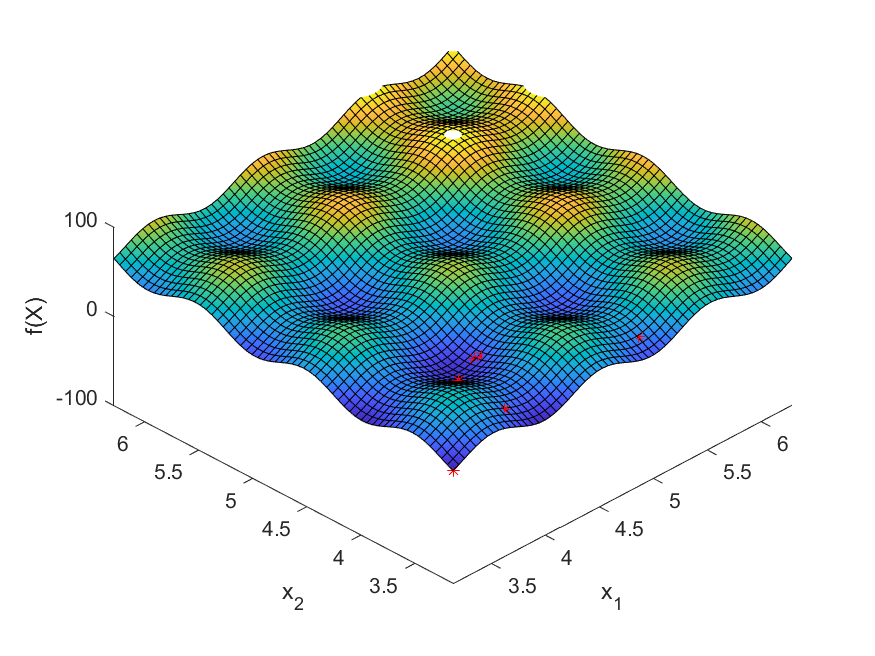
\includegraphics[width=0.65\textwidth]{img/smpl/rast2dshft/loa-iter-50}
    \caption{Iteration 50}
  \end{center}
  \end{figure}
\end{frame}

\begin{frame}{CEC 2014 Benchmarks}
  Each year CEC provides a set of functions that are known for testing optimization algorithms for scientists to submit their work and compare the effectiveness of their algorithms. The code is reviewable and written in C++ and adapted to compatible languages.
\end{frame}
\begin{frame}{CEC 2014 Benchmarks}
  Each year CEC provides a set of functions that are known for testing optimization algorithms for scientists to submit their work and compare the effectiveness of their algorithms. The code is reviewable and written in C++ and adapted to compatible languages.
\end{frame}

\begin{frame}{CEC 2014 Benchmarks}
\begin{table}[]
\resizebox{\textwidth}{!}{
\begin{tabular}{llll}
  \textbf{Type}
    & \textbf{ID} & \textbf{Function} & \textbf{f*} \\ \hline
  Unimodal
    & f1 & Rotated high conditioned elliptic function & 100 \\
    & f2 & Rotated bent cigar function & 200 \\
    & f3 & Rotated discus function & 300 \\
  Multimodal
    & f4 & Shifted and rotated Rosenbrock function & 400 \\
    & f5 & Shifted and rotated Ackley's function & 500 \\
    & f6 & Shifted and rotated Weierstrass function & 600 \\
    & f7 & Shifted and rotated Griewank's function & 700 \\
    & f8 & Shifted Rastrigin function & 800 \\
    & f9 & Shifted and rotated Rastrigin's function & 900 \\
    & f10 & Shifted Schwefel function & 1000 \\
    & f11 & Shifted and rotated Schwefel's function & 1100 \\
    & f12 & Shifted and rotated Katsuura function & 1200 \\
    & f13 & Shifted and rotated HappyCat function & 1300 \\
    & f14 & Shifted and rotated HGBat function & 1400 \\
    & f15 & Shifted and rotated Expanded Griewank's plus Rosenbrock's function & 1500 \\
    & f16 & Shifted and rotated Expanded Scaffer's F6 function & 1600 \\
\end{tabular}}
\caption{Functions defined by CEC 2014 and used for testing}
\end{table}
\end{frame}

\begin{frame}{CEC 2014 Benchmarks}
\begin{table}[]
\resizebox{\textwidth}{!}{
\begin{tabular}{llll}
  \textbf{Type}
    & \textbf{ID} & \textbf{Function} & \textbf{f*} \\ \hline
  Hybrid
    & f17 & Hybrid function1 (f 9, f 8, f 1) & 1700 \\
    & f18 & Hybrid function2 (f 2, f 12, f 8) & 1800 \\
    & f19 & Hybrid function3 (f 7, f 6, f 4, f 14) & 1900 \\
    & f20 & Hybrid function4 (f 12, f 3, f 13, f 8) & 2000 \\
    & f21 & Hybrid function5 (f 14, f 12, f 4, f 9, f 1) & 2100 \\
    & f22 & Hybrid function6 (f 10, f 11, f 13, f 9, f 5) & 2200 \\
  Composition
    & f23 & Composition function1 (f 4, f 1, f 2, f 3, f 1) & 2300 \\
    & f24 & Composition function2 (f 10, f 9, f 14) & 2400 \\
    & f25 & Composition function3 (f 11, f 9, f 1) & 2500 \\
    & f26 & Composition function4 (f 11, f 13, f 1, f 6, f 7) & 2600 \\
    & f27 & Composition function5 (f 14, f 9, f 11, f 6, f 1) & 2700 \\
    & f28 & Composition function6 (f 15, f 13, f 11, f 16, f 1) & 2800 \\
    & f29 & Composition function7 (f 17, f 18, f 19) & 2900 \\
    & f30 & Composition function8 (f 20, f 21, f 22) & 3000
\end{tabular}}
\caption{Functions defined by CEC 2014 and used for testing}
\end{table}
\end{frame}

\begin{frame}{CEC 2014 Benchmarks}
The benchmark ran 60 times of the algorithm on each function totalling to 30 functions. The limit placed to stop the algorithm is when it reaches 150,000 function evaluations.
\end{frame}

\begin{frame}{CEC 2014 Benchmarks}
\begin{table}[]
\resizebox{0.6\textwidth}{!}{
\begin{tabular}{lllll}
    & min                               & max                               & std                               & median                            \\
f1  & \cellcolor[HTML]{FD6864}1.647E+07 & \cellcolor[HTML]{FD6864}6.730E+07 & \cellcolor[HTML]{FD6864}1.053E+07 & \cellcolor[HTML]{FD6864}3.844E+07 \\
f2  & \cellcolor[HTML]{FD6864}2.645E+05 & \cellcolor[HTML]{FD6864}6.888E+06 & \cellcolor[HTML]{FD6864}1.386E+06 & \cellcolor[HTML]{FD6864}2.092E+06 \\
f3  & \cellcolor[HTML]{67FD9A}1.034E+04 & \cellcolor[HTML]{67FD9A}3.092E+04 & \cellcolor[HTML]{67FD9A}3.979E+03 & \cellcolor[HTML]{67FD9A}1.670E+04 \\
f4  & \cellcolor[HTML]{67FD9A}4.738E+02 & \cellcolor[HTML]{67FD9A}6.284E+02 & \cellcolor[HTML]{67FD9A}3.272E+01 & \cellcolor[HTML]{67FD9A}5.611E+02 \\
f5  & \cellcolor[HTML]{67FD9A}5.208E+02 & \cellcolor[HTML]{67FD9A}5.210E+02 & \cellcolor[HTML]{67FD9A}5.124E-02 & \cellcolor[HTML]{67FD9A}5.210E+02 \\
f6  & \cellcolor[HTML]{67FD9A}6.195E+02 & \cellcolor[HTML]{67FD9A}6.296E+02 & \cellcolor[HTML]{67FD9A}2.167E+00 & \cellcolor[HTML]{67FD9A}6.254E+02 \\
f7  & \cellcolor[HTML]{67FD9A}7.005E+02 & \cellcolor[HTML]{67FD9A}7.011E+02 & \cellcolor[HTML]{67FD9A}1.218E-01 & \cellcolor[HTML]{67FD9A}7.009E+02 \\
f8  & \cellcolor[HTML]{67FD9A}8.547E+02 & \cellcolor[HTML]{67FD9A}9.298E+02 & \cellcolor[HTML]{67FD9A}1.350E+01 & \cellcolor[HTML]{67FD9A}8.845E+02 \\
f9  & \cellcolor[HTML]{67FD9A}9.658E+02 & \cellcolor[HTML]{67FD9A}1.028E+03 & \cellcolor[HTML]{67FD9A}1.518E+01 & \cellcolor[HTML]{67FD9A}9.971E+02 \\
f10 & \cellcolor[HTML]{67FD9A}2.586E+03 & \cellcolor[HTML]{67FD9A}7.135E+03 & \cellcolor[HTML]{67FD9A}1.273E+03 & \cellcolor[HTML]{67FD9A}3.864E+03 \\
f11 & \cellcolor[HTML]{67FD9A}3.717E+03 & \cellcolor[HTML]{67FD9A}8.245E+03 & \cellcolor[HTML]{67FD9A}1.148E+03 & \cellcolor[HTML]{67FD9A}7.470E+03 \\
f12 & \cellcolor[HTML]{67FD9A}1.202E+03 & \cellcolor[HTML]{67FD9A}1.203E+03 & \cellcolor[HTML]{67FD9A}3.312E-01 & \cellcolor[HTML]{67FD9A}1.203E+03 \\
f13 & \cellcolor[HTML]{67FD9A}1.300E+03 & \cellcolor[HTML]{67FD9A}1.301E+03 & \cellcolor[HTML]{67FD9A}8.465E-02 & \cellcolor[HTML]{67FD9A}1.300E+03 \\
f14 & \cellcolor[HTML]{67FD9A}1.400E+03 & \cellcolor[HTML]{67FD9A}1.400E+03 & \cellcolor[HTML]{67FD9A}3.087E-02 & \cellcolor[HTML]{67FD9A}1.400E+03 \\
f15 & \cellcolor[HTML]{67FD9A}1.514E+03 & \cellcolor[HTML]{67FD9A}1.549E+03 & \cellcolor[HTML]{67FD9A}7.715E+00 & \cellcolor[HTML]{67FD9A}1.525E+03 \\
\end{tabular}}
\end{table}
\end{frame}

\begin{frame}{CEC 2014 Benchmarks}
\begin{table}[]
\resizebox{0.6\textwidth}{!}{
\begin{tabular}{lllll}
    & min                               & max                               & std                               & median                            \\
f16 & \cellcolor[HTML]{67FD9A}1.611E+03 & \cellcolor[HTML]{67FD9A}1.613E+03 & \cellcolor[HTML]{67FD9A}3.086E-01 & \cellcolor[HTML]{67FD9A}1.612E+03 \\
f17 & \cellcolor[HTML]{FD6864}5.180E+05 & \cellcolor[HTML]{FD6864}3.363E+06 & \cellcolor[HTML]{FD6864}5.823E+05 & \cellcolor[HTML]{FD6864}1.612E+06 \\
f18 & \cellcolor[HTML]{67FD9A}1.991E+03 & \cellcolor[HTML]{67FD9A}1.350E+04 & \cellcolor[HTML]{67FD9A}2.131E+03 & \cellcolor[HTML]{67FD9A}2.910E+03 \\
f19 & \cellcolor[HTML]{67FD9A}1.911E+03 & \cellcolor[HTML]{67FD9A}1.923E+03 & \cellcolor[HTML]{67FD9A}2.082E+00 & \cellcolor[HTML]{67FD9A}1.919E+03 \\
f20 & \cellcolor[HTML]{67FD9A}4.630E+03 & \cellcolor[HTML]{67FD9A}2.635E+04 & \cellcolor[HTML]{67FD9A}4.406E+03 & \cellcolor[HTML]{67FD9A}1.484E+04 \\
f21 & \cellcolor[HTML]{FD6864}7.908E+04 & \cellcolor[HTML]{FD6864}7.593E+05 & \cellcolor[HTML]{FD6864}1.624E+05 & \cellcolor[HTML]{FD6864}2.698E+05 \\
f22 & \cellcolor[HTML]{67FD9A}2.473E+03 & \cellcolor[HTML]{67FD9A}3.134E+03 & \cellcolor[HTML]{67FD9A}1.545E+02 & \cellcolor[HTML]{67FD9A}2.782E+03 \\
f23 & \cellcolor[HTML]{67FD9A}2.620E+03 & \cellcolor[HTML]{67FD9A}2.633E+03 & \cellcolor[HTML]{67FD9A}2.678E+00 & \cellcolor[HTML]{67FD9A}2.624E+03 \\
f24 & \cellcolor[HTML]{67FD9A}2.618E+03 & \cellcolor[HTML]{67FD9A}2.632E+03 & \cellcolor[HTML]{67FD9A}3.211E+00 & \cellcolor[HTML]{67FD9A}2.627E+03 \\
f25 & \cellcolor[HTML]{67FD9A}2.700E+03 & \cellcolor[HTML]{67FD9A}2.709E+03 & \cellcolor[HTML]{67FD9A}2.528E+00 & \cellcolor[HTML]{67FD9A}2.707E+03 \\
f26 & \cellcolor[HTML]{67FD9A}2.700E+03 & \cellcolor[HTML]{67FD9A}2.701E+03 & \cellcolor[HTML]{67FD9A}1.122E-01 & \cellcolor[HTML]{67FD9A}2.700E+03 \\
f27 & \cellcolor[HTML]{67FD9A}3.117E+03 & \cellcolor[HTML]{67FD9A}3.739E+03 & \cellcolor[HTML]{67FD9A}1.630E+02 & \cellcolor[HTML]{67FD9A}3.536E+03 \\
f28 & \cellcolor[HTML]{67FD9A}3.255E+03 & \cellcolor[HTML]{67FD9A}4.404E+03 & \cellcolor[HTML]{67FD9A}1.954E+02 & \cellcolor[HTML]{67FD9A}3.296E+03 \\
f29 & \cellcolor[HTML]{67FD9A}3.125E+03 & \cellcolor[HTML]{67FD9A}4.300E+03 & \cellcolor[HTML]{67FD9A}1.531E+02 & \cellcolor[HTML]{67FD9A}3.131E+03 \\
f30 & \cellcolor[HTML]{67FD9A}3.813E+03 & \cellcolor[HTML]{67FD9A}7.945E+04 & \cellcolor[HTML]{67FD9A}1.646E+04 & \cellcolor[HTML]{67FD9A}4.796E+03
\end{tabular}}
\end{table}
\end{frame}

\begin{frame}{CEC 2014 Benchmarks: Run-Time vs Fitness}
%--dito
\end{frame}

\begin{frame}{Conclusion}
The Lion Optimization Algorithm uses a Lion-Pride-Outcast behavior for a population to find solutions or what is thought of as a better territory or a safer place for the population to live in. It utilizes a combination of multiple popular optimization techniques like GA to improve on solutions.
\end{frame}
%------------------------------------------------

\end{document}
